\documentclass[twocolumn,tighten]{aastex62}
\turnoffedit 

\shorttitle{Hz-Dyn}
\shortauthors{Xue et al.}


%%%%%%%%%%%%%%%%%%%%%%%%%%%%%
%	load package
%%%%%%%%%%%%%%%%%%%%%%%%%%%%%

\usepackage[us,12hr]{datetime}
\usepackage{graphicx}
\usepackage{gensymb}
\usepackage{listings}
\usepackage{color}
\usepackage{mathrsfs}
\usepackage{natbib}
\usepackage{booktabs}
\usepackage{comment}
\usepackage{morefloats}
\usepackage{sidecap}
\usepackage{grffile}
\usepackage{verbatim}
\usepackage{longtable}
\usepackage{etoolbox}
\usepackage{amsmath}

\DeclareMathOperator{\sech}{sech}
\DeclareMathOperator{\csch}{csch}
%\DeclareMathOperator{\arcsec}{arcsec}
%\DeclareMathOperator{\arccot}{arcCot}
%\DeclareMathOperator{\arccsc}{arcCsc}
%\DeclareMathOperator{\arccosh}{arcCosh}
%\DeclareMathOperator{\arcsinh}{arcsinh}
%\DeclareMathOperator{\arctanh}{arctanh}
%\DeclareMathOperator{\arcsech}{arcsech}
%\DeclareMathOperator{\arccsch}{arcCsch}
%\DeclareMathOperator{\arccoth}{arcCoth} 


\usepackage{amssymb}
\usepackage{catchfilebetweentags}
\usepackage{multirow}

\newcommand{\kms}{\mbox{$\rm km\,s^{-1}$}}

\newcommand{\citwo}{\mbox{{\rm [\ion{C}{1}]$\,{{^3P_2}\to{^3P_1}}$}}}

\newcommand{\cione}{\mbox{{\rm [\ion{C}{1}]$\,{{^3P_1}\to{^3P_0}}$}}}
\newcommand{\coone}{\mbox{${\rm CO\,{\it J}=1\to0}$}}
\newcommand{\cotwo}{\mbox{${\rm CO\,{\it J}=2\to1}$}}
\newcommand{\cothree}{\mbox{${\rm CO\,{\it J}=3\to2}$}}
\newcommand{\cofour}{\mbox{${\rm CO\,{\it J}=4\to3}$}}
\newcommand{\coseven}{\mbox{${\rm CO\,{\it J}=7\to6}$}}
\newcommand{\lya}{\mbox{\rm Ly$\alpha$}}
\newcommand{\msun}{\mbox{$M_{\odot}$ }}


% lanaguages

\newcommand{\python}{{\sc python}}
\newcommand{\idl}{{\sc IDL}}

% codes

\newcommand{\gmake}{{\tt GMaKE}}
\newcommand{\clean}{{\scshape clean}}
\newcommand{\kinms}{{\tt KinMS}}
\newcommand{\galpy}{{\tt galpy}}
\newcommand{\galario}{{\tt galario}}
\newcommand{\emcee}{{\tt emcee}}
\newcommand{\lmfit}{{\tt lmfit}}
\newcommand{\galfit}{{\tt galfit}}
\newcommand{\pycasacore}{{\tt python-casacore}}
\newcommand{\casacore}{{\tt casacore}}
\newcommand{\pyfftw}{{\tt py-fftw}}
\newcommand{\scipyfftw}{{\tt scipy-fftw}}
\newcommand{\mklfft}{{\tt Intel MKL-FFT}}
\newcommand{\barolo}{{\tt $^{\rm 3D}$Barolo}}
\newcommand{\galpak}{{\tt GalPak$^{\rm 3D}$}}
\newcommand{\tirific}{{\tt TiRiFiC}}
\newcommand{\galmod}{{\tt GIPSY/GALMOD}}

\begin{document}

\title{\gmake: Galaxy Morphology and Kinematics Estimator}

\author[0000-0001-7689-9305]{Rui Xue}
\affiliation{Department of Physics \& Astronomy, University of Iowa, 203 Van Allen Hall, Iowa City, IA 52242, USA}

\author[0000-0001-9608-6395]{Hai Fu}
\affiliation{Department of Physics \& Astronomy, University of Iowa, 203 Van Allen Hall, Iowa City, IA 52242, USA}

%\author[0000-0001-9608-6395]{Friends}
%\affiliation{TBD}

\begin{abstract}

GMaKE is a toolkit for evaluating galaxy morpgology and kinnemtics from astronomical 2D images or 3D spectral cubes.
It take the advantages of various existing programs for galaxy modeling and essentially severe as a flexible wrapper for quatifying the galaxy geometry and kinematics structures through parameterized models, with varieties of parameter fitting and error estimation algorithm to choose from. 
%Advantages compared with the other codes:
With a flexible modulated code design, the toolkit can easily incorporate an arbitrary galaxy emission models with a proper adapter and perform parameter optimization to search for most proper model solutions.\\
With the modern interferometer dataset in mind, the model-data comparison can be performed in either spatial or visibility domain, which avoid the no-linear effect in image deconvolution.\\
Because we construct synthetical radio/optical spectral or continuum images at different wavelengths/frequencies using realistic instrumental response functions from a galaxy model characterized by shared physical geometry and independent line/continuum emissivity functions, the code is capable to fit all available data with a unified model, even under the complicated situation in which the data are contributed by multiple blending objects and absorptions/emission lines.




\end{abstract}

\keywords{
galaxies: formation ---
galaxies: structure --
galaxies: kinematics ---
methods: data analysis}

\tableofcontents

\section{Introduction}

% this is a framework

% importance of galaxy kinematics and morphology galaxies

A fundamental aspect of the galaxy evolution study is to understand their dynamical structure and matter distributions. 
The majority of such information comes from their electromagnetic radiation: the emission and absorption at different wavelength can trace various matter components at certain physical conditions, along the line of sight; while spectral line features can further reveal the galaxy kinematics through the Doppler shift.
Therefore, the kinematic and morphological analyses based on spectroscopy or imaging are the essential technique for galaxy study.

% Tools are needed but the ones on the market show limitations

While many specialized tools have been developed for such measurement in last decades to overcome the limitations of resolution and sensitivity inherent in the observed data, we have identified two major limitations in existing development: 1) many programs are focused on the application based on a single data set or type;
2) most codes are exclusively designed for either continuum or spectral line emission (even restricted to a single object or one line component).
The former design limits the joint constrain power from multi-wavelength datasets in different forms (e.g., images, slit-spectroscopy, etc.), which become widely available in the modern astronomy "big-data" era. 
The latter coding principle unnecessarily requires the original dataset to be decomposed before any analysis. As object/line belending and coexisting of line and continuum emission are common in astronomical data, this additional layer of data manipulation introduce uncertain especially in low SNR conditions.

\gmake\\footnote{\url{https://github.com/r-xue/GMaKE}} is a Python-based modeling code for evaluating galaxy morphology and kinematics 
from multiple-band astronomical observations.
\gmake\ first builds an intrinsic galaxy line and/or continuum emission model based on the parameterized spatial and kinematical models of different components, and then pass the result to simulated observations to generate mockup data, which can be directly compared with observational datasets.
Different from previous fitting algorithms which were usually applied to 2-dimension single dataset, our fitting method can be simultaneously applied to multiple datasets obtained in different forms (e.g., images, spectral-cubes, or interferometric visibilities).
The forward-modeling approach can not only provide a joint constraint from all available observational evidence at different spatial/spectral resolutions, but also simplify the model uncertainty estimation by minimizing advanced data manipulations (e.g., continuum subtraction for diffuse line emission, interferometry imaging/\clean of low-SNR data without zero-spacing information).

While this is not the first program fitting spectral cube, the code is designed to offer some uniq advantages:

\begin{itemize}
\item Different Model Fitting Methods, emcee, amoeba
\item Visibility DataSet
\item Friendly parameter format
\item Physical Models
\end{itemize}
%low-intensity diffuse emission 
%CLEAN depth/weights
%as long as the noise chractertistics 
%is straighfordwardly quantified in each dataset. 
% despite the reliaon on prior (parametrized sptial and kinmeticall models for different emission components), with prior physically-motivated prior assumption, the algoirthm is ideal extract morphplgy and kinematics information for moderately resolved and low-SNR datasets which is common for high-redshift objects.

The paper is organized as follows.
We present the philosophical principle of our code design and technical details in Section\,2. It is followed with multiple application examples fron Section\,3: a rich multi-wavelenth datasets of normal start-forming high-redshift galaxy, including both ALMA radio and IFU IR data; a sythetica moderatedly resolved galaxy based on high-resolution nearby galaxy dataset; a high-z galaxy with rest-frame \lya\ and UV imaging. Section 4 compares the algorithm with previous modeling methods. Finally, we summarize the future perspective of expanding capabilty and application of \gmake. 



\section{Modeling Overview}


In this section, we give a quick overview of \gmake\ workflow.

One important design choice in \gmake\ is that we built emission model on the physical dimension and then transform the emission into the native data form obtained in observations. 
Therefore, the application will require that the data were provide along with correct WCS system or observational metadata (e.g., u-v sampling in interfemeteric data)

\begin{figure*}%[h!]
\centering
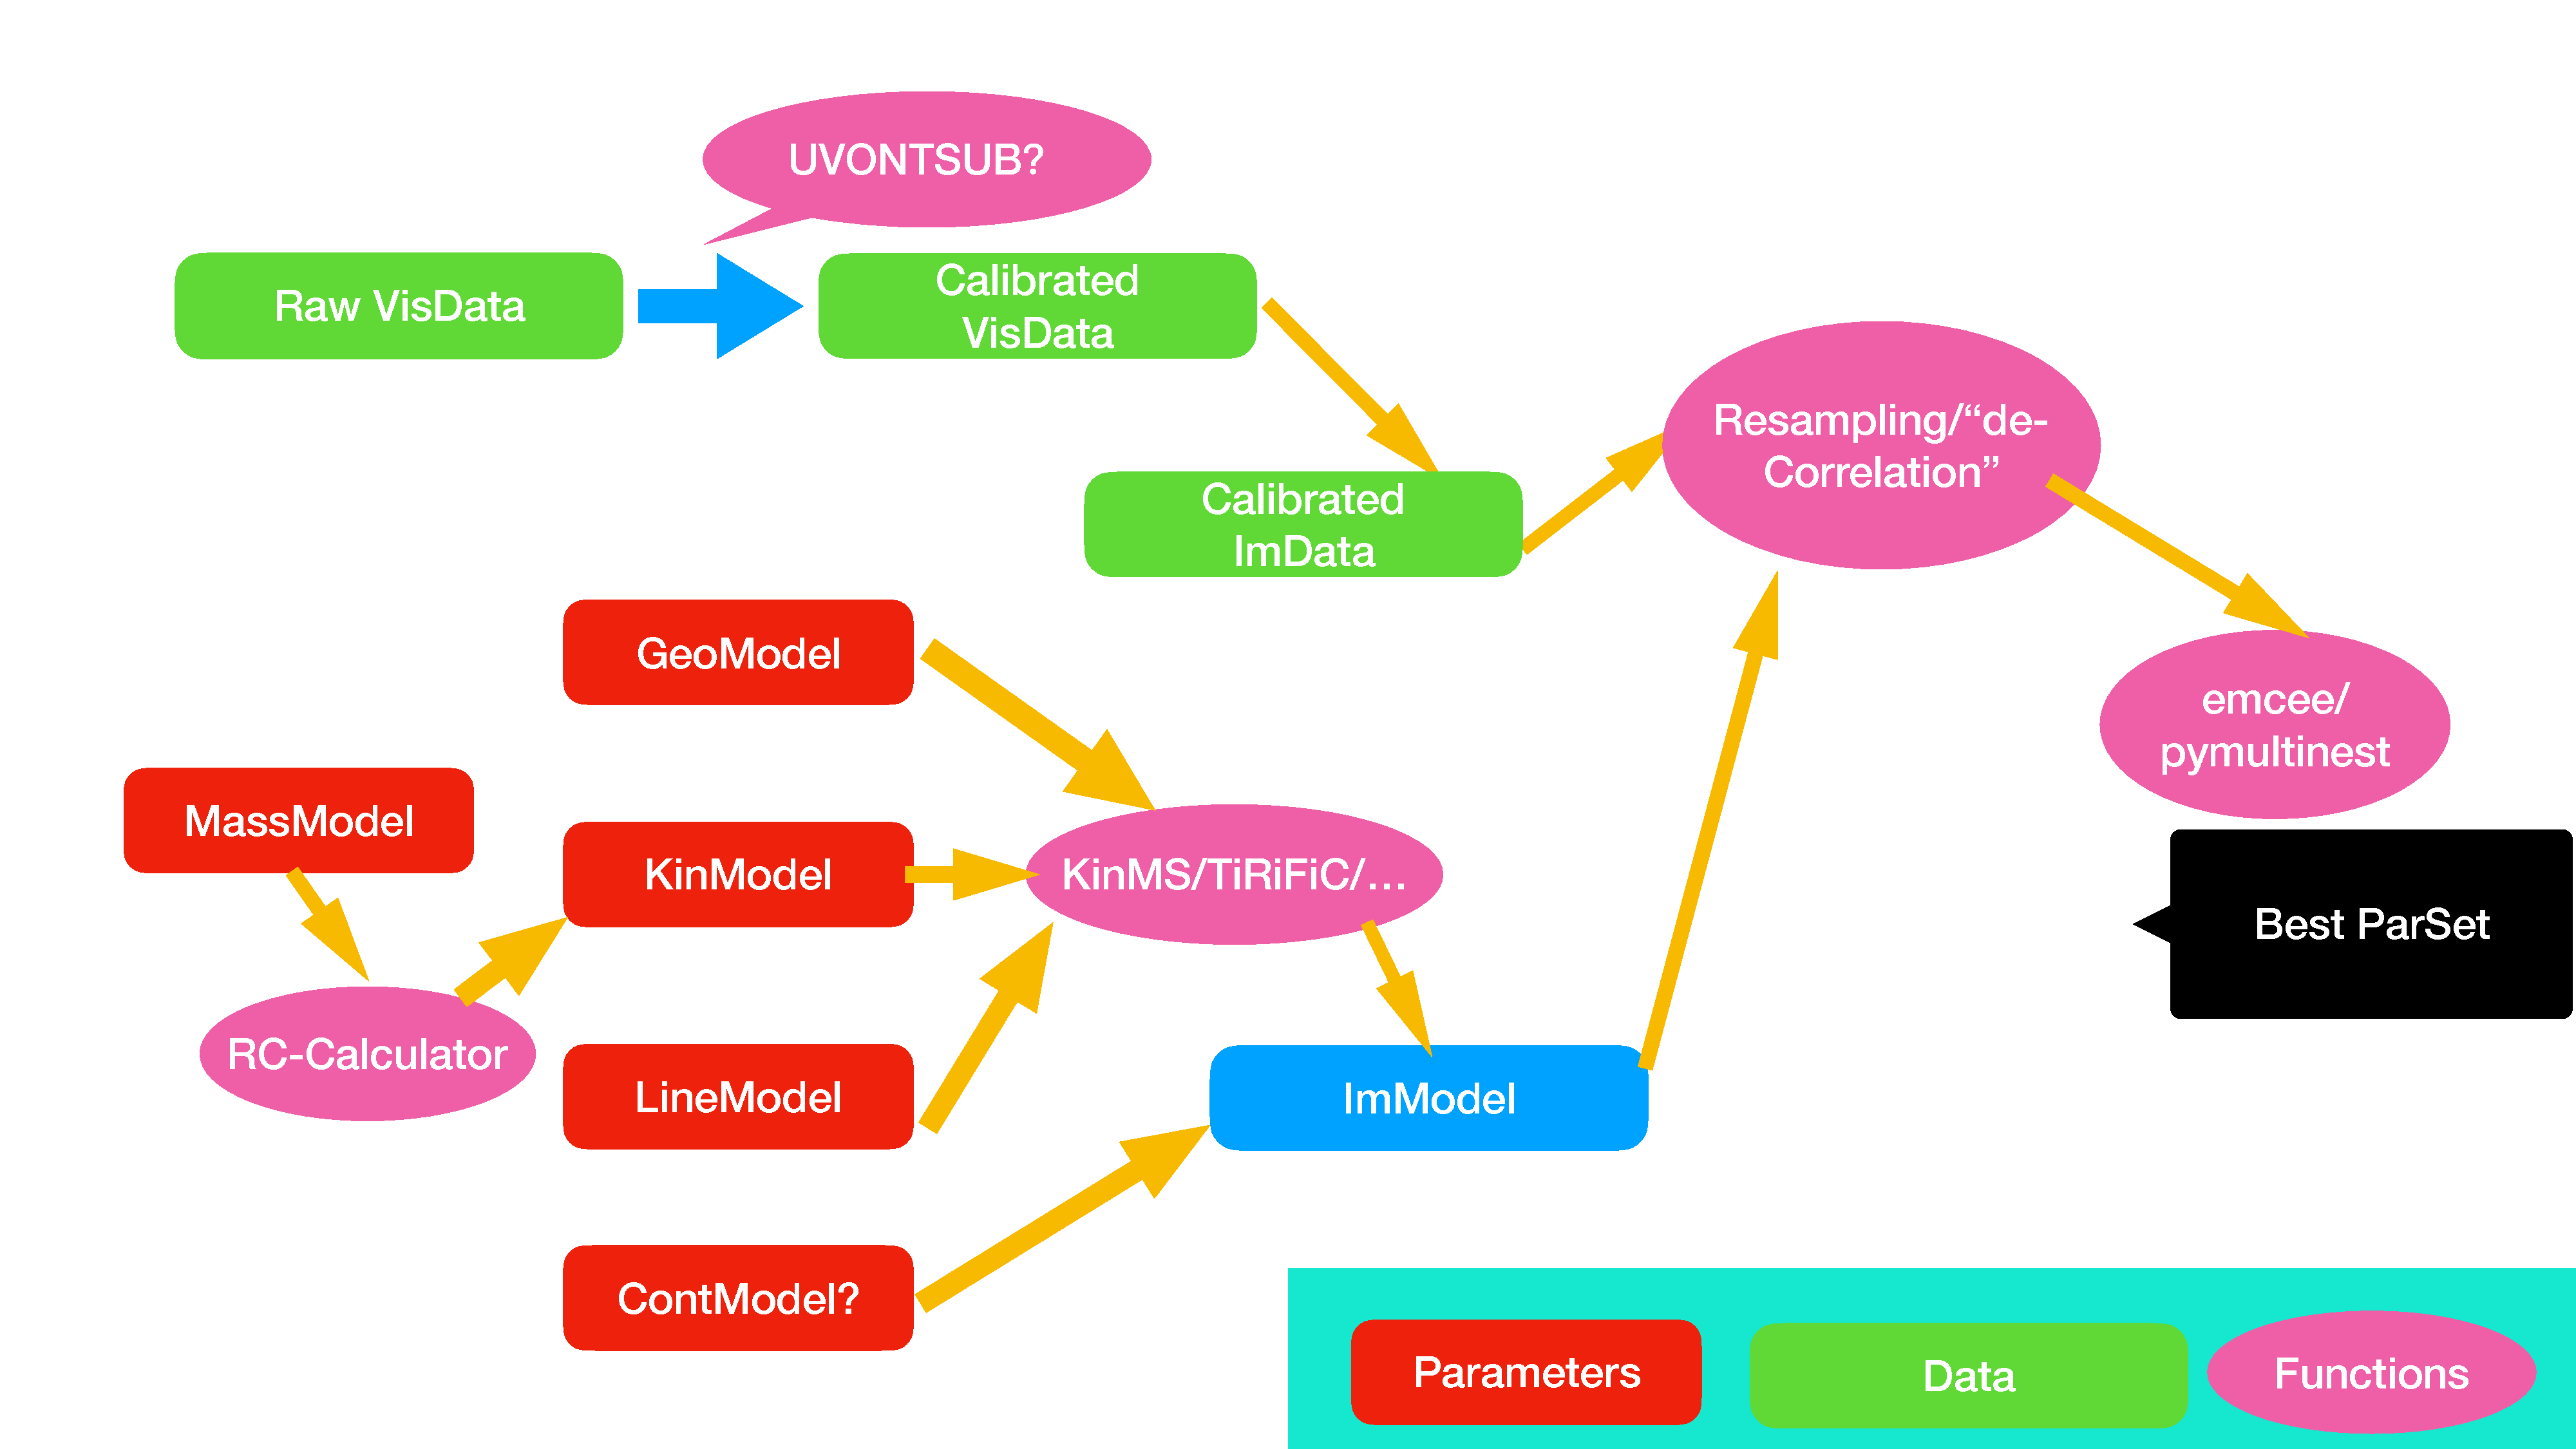
\includegraphics[width=0.48\textwidth]{figures/pipeline-workflow-im.pdf}
%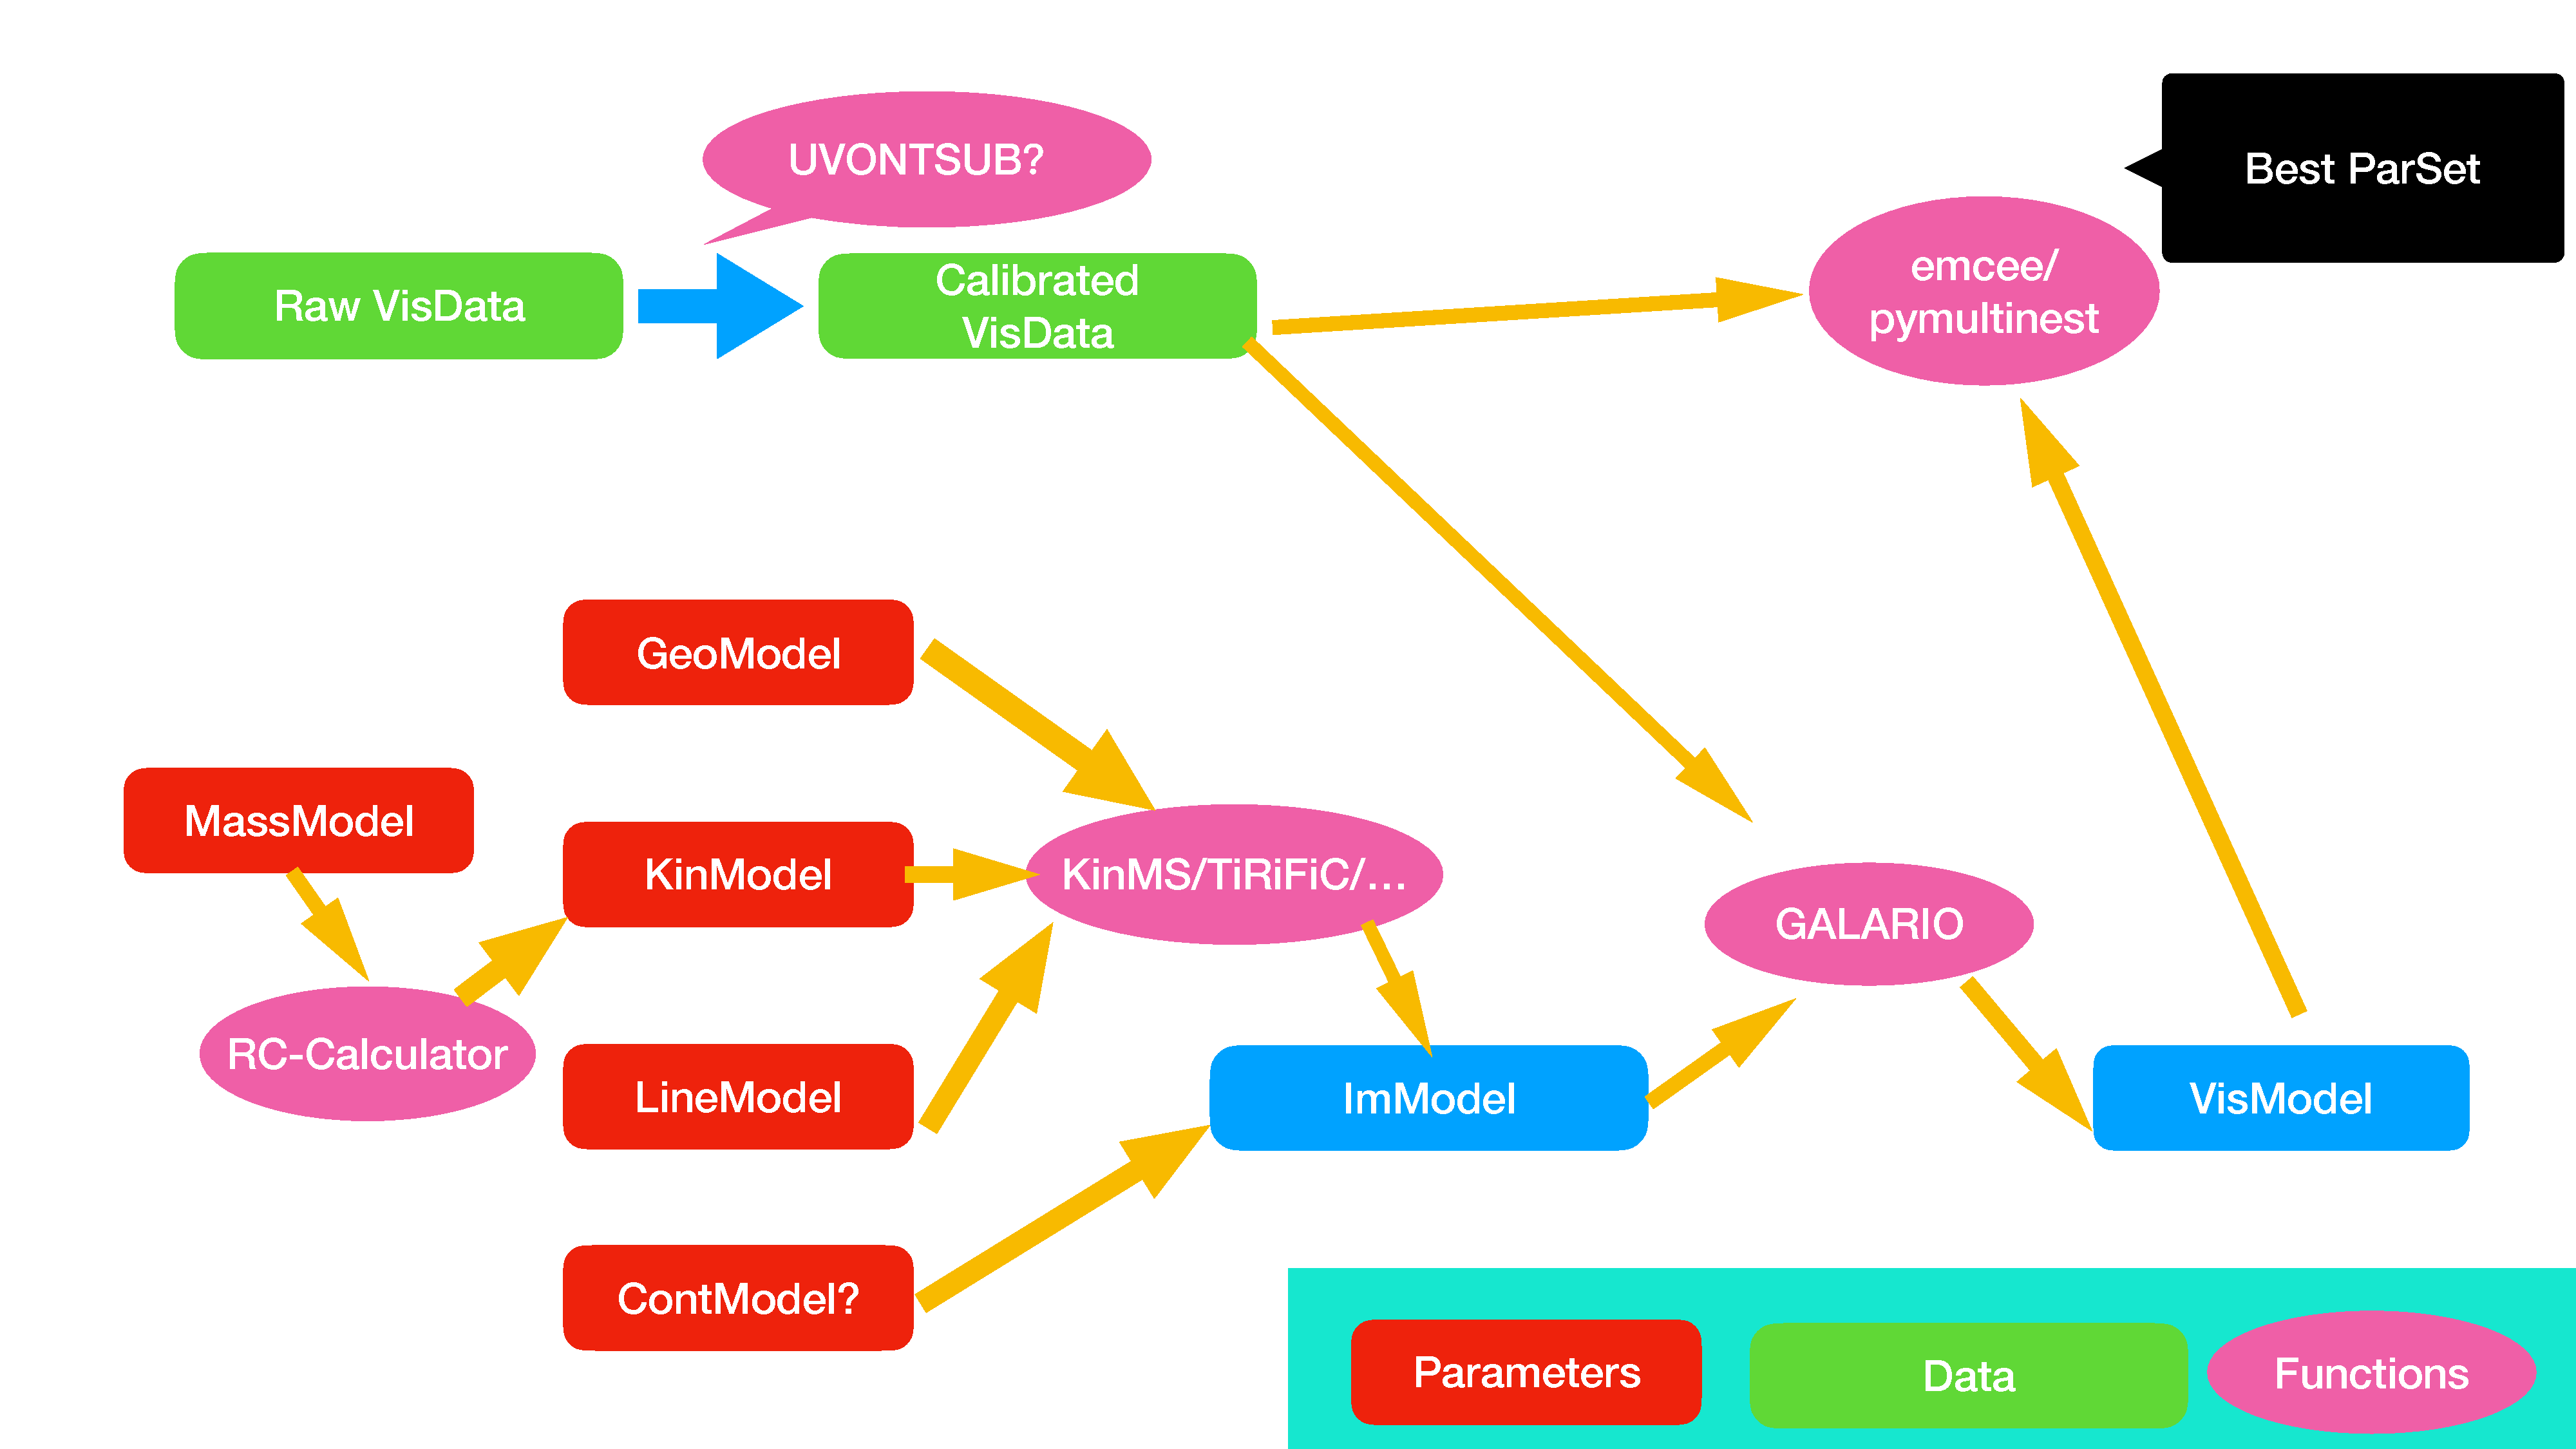
\includegraphics[width=0.48\textwidth]{figures/pipeline-workflow-vis.pdf}
\caption{code structure/workflow: xy-version/uv-version
\label{fig:spec}
}
\end{figure*}

We recap some feature but empherize what we improved.


\subsection{Spectral Line Emission}

To model spatially resolved spectral line emission of galaxies, we require a parameterized prescription for the line emissivity and galaxy kinematic structures.
We start with a first-order base model by assuming the line emission arises from an axial-symmetry disk morphology with organized rotation. The second-order morphology alternation or other motion components can be added upon it.
In this section, we describe the geometry and kinematics setup in our models, with second-order features described at the end.

\subsubsection{Geometry and Emissivity Model}

We set up a 3D Cartesian coordinate system with the presumed galactic disk on the ($x$, $y$) plane.
The emissivity distribution is parameterized as $I(r,z)$, which depends on the galactocentric distance $r=\sqrt{x^2+y^2}$ and the above-plane height $z$. The default option is,
\begin{eqnarray}\label{eq:rp}
I(r,z) & = & I(r)I(z)  \\
    & \propto     & \exp\left\{-b_{\rm n}\left[\left(\frac{r}{r_{\rm e}}\right)^{1/n}-1\right]\right\} \exp\left(-\frac{z^2}{2h_{\rm z}^2}\right) 
%    &            & 
\end{eqnarray}
This presents a \citet{Sersic:1963aa} surface brightness (SB) radial profile with a half-light radius of $r_{\rm e}$ and a S{\'e}rsic index of $n$.
In addition, it assumes a Gaussian brightness distribution perpendicular to the galactic plane with a characteristic disk thickness of $h_{\rm z}$.
The $b_{\rm n}$ value in the radial profile component will depend on the S{\'e}rsic index. A Gaussian profile, an exponential profile \citep{Freeman:1970eb}, or the classic \cite{de-Vaucouleurs:1948aa} profile, can be obtained by fixing the S{\'e}rsic index $n=0.5$, $1$, or $4$, with the corresponding $b_{n}$ value of 0.686, 1.678, and 7.669, respectively.

Our program also allows users to adopt arbitrary radial or vertical profile analytical forms through an algebraic expression in parameters files (see Section\,\ref{sec:fitting} and Table\,\ref{tb:rc_examples} for more details). 
In addition, some common analytical radial/vertical profile functions are written as built-in options,
such as the $\sech^2\left(z/2h_{\rm z}\right)$ ``isothermal'' vertical distribution \citep{van-der-Kruit:1981aa} or a more general form from \citet{van-der-Kruit:1988aa},
\begin{eqnarray}\label{eq:vp}
I(z)\propto\sech^{2/n}\left(\frac{nz}{2h_{\rm z}}\right).
\end{eqnarray}


\subsubsection{Kinematic and Dynamical Model}

The model kinematical structure is also specified in the same Cartesian coordinate system.
The default option is described by a well-organized rotation with a rotational velocity depending on the galactocentric distance.
% ordered
The rotation curve can be specified as a tabulated radial profile, an analytical function form. 

We also provide an option of using a rotation curve derived from 
a dynamical model, which is based on the gravitational potential of specified disk/halo-like mass distributions (see Table\,\ref{tb:rc_examples}).
In this option, the parameter set describing mass distributions is translated into a gravitational potential model using the \python\ module \galpy\ \citep{Bovy:2015aa}, which also calculates the rotational velocity expected on the galactic plane.
The mass distribution can be described by mass components mimicking the common galactic disk or DM halo distribution, or directly scaled from the disk-plane light distribution using a constant light-to-mass ratio.

The velocity dispersion is assumed to be uniform in the galaxy by default, although a radial or vertical dependency can be added.
The potential-based dynamical model does not account of the dispersion-based support to the disk, therefore it's only strictly correct if the ratio of bulk rotation velocity $v_{\rm rot}$ to the turbulent motion $\sigma_{v}$ is significantly larger than unity (i.e., rotation-dominated rather than pressure-supported), which may be not rule for high-$z$ disks and current observations
become unable to differentiate between pressure-supported and
rotation-dominated galaxies (see, e.g., Tamburro et al. 2009
and Stilp et al. 2013).

%\subsection{Continuum Emission}
%\subsubsection{2D Dirtibution Model in the SkyPlan coodrinate}
%
%Rotational Disk, or Parametrized RC, or Gravitational Motived RC, or RC built upon the Light-Mass Distribution. Continuum Models. Independence of galaxy Orientation.

%\subsubsection{Advanced manuiulayion}
%
%SinTerm / inflow.
%
%Use 2D prior


%\subsubsection{Opacity Model / Line of Sign obscution}
%
%Add the opacity...


\subsubsection{Emission Model in the ($\alpha, \delta, v/\nu/\lambda$) domain}

We follow the Monte Carlo approach to produce a spectral cube model. 
The procedure essentially generates a set of ``cloudlets", with their spatial positions and velocity vectors randomly assigned following the specified galaxy morphology and kinematics structure distribution. After a spatial-to-sky coordination transform, and they are integrated into a position-position-velocity (PPV) space using their on-sky position and the line-of-sight velocity components. The same ``tilted-ring'' principal \citep{Rogstad:1974aa} is adopted for other similar modeling codes such as \galmod,
\barolo, or \tirific\ \citep{van-der-Hulst:1992aa,Jozsa:2007aa,Di-Teodoro:2015aa,Bouche:2015aa}

The coordinate transformation in our program requires the geometry setup of the ($x$,$y$) plane relative to the sky plane ($\alpha$, $\delta$), which include the ($x$, $y$) plane origin in WCS coordinates, the inclination of the ``ring'' and position angle of the major axis of its on-sky projection.
The line-of-sight radial velocity can be further transformed into the wavelength of frequency of spectral lines when the galaxy systematic velocity (or its redshift) and rest-wavelength/frequency are provided.
%Due to the random process, a discretization noise exists in the model spectral cube, which is               proportional to the square root of the number of cloudlets added into a pixel in the data cube. 
%For continuum emission, the input include a parameterized brightness distribution (e.g. GalFIT like options) \citep{Peng:2010eh} and a wavelength/frequency dependency of integrated flux. 
%For line emission, the projected emission distribution is build from a tiled-disk model or a more general complex mopholgym, a tiled-disk kinematics is assumed (usually radial profile dependent), and a 3D spectral cube is contrunstuced. The underline algorithm was built upon a extensely modified code based on the KinMS routine \citep{Davis:2013aa}.

We design the program to model multiple emission components and objects. At the same time, all emission components are integrated and mapped into different datasets through simulated observation described below.
%are then added into a spectral-cube for observational simulation.
%An extinction model can also be included.
%It is also possible to build an intrinsic model from external program.
%Gas kinmectis is approximated by the tilte-ring model (Rogstad+1974), i.e., a galactic disk at the location galactocentric radius with kinematics approximation by a circular rotation velocity and gas dispension, which are dependent on 
%If mutiple object is set as input, all of them will be mapped into the data coordinate system.
%If mutiple dataset is proviedm the emission model will be mapped into each of then for a joint model fitting.

\subsection{Simulated Observations}

One critical design goal of \gmake\ is the implementation of forward modeling approach:
The models will be mapped into the observational datasets for parameter fitting through simulated observations.
Depending on the types of observation and the data format, the simulation will require different metadata and call different subroutines compoents. 
We describe the mapping process details for three supported types of data in this section.

\subsubsection{Visibility}

The program is able to directly read the radio interferometric visibility data stored in the CASA Measurement Set (MS) format\footnote{\url{https://casa.nrao.edu/Memos/229.html};\cite{van-Diepen:2015aa}} using the \pycasacore\footnote{\url{http://casacore.github.io/python-casacore/}} module.
\pycasacore\ provides a \python\ interface to the \casacore\ library, which is standalone from the CASA package. 
 It allows direct access and manipulation of the essential information stored in MS tables, including the complex visibility data, $u$-$v$ coordinates, and weights.
We convolve the intrinsic spectral cube or image model with the telescope primary beam, and then transfer the results into a visibility model with the $u$-$v$ coordinates from MS tables, using \galario\ \citep{Tazzari:2018aa}.
The visibility model is then exported to the MS model column for evaluation or imaging.
While the current implementation only supports MS, the program should also work if a proper data conversion is done.
%as the visibility format as it is widely available for radio interferometers (e.g. ALMA, VLA)

%A statcical noise is re-calculated 
%Two gooodness is created:
%Eviden likelyhood:
%
%which can be used for different fitting algorithm.

\subsubsection{Spectral-Cube/Image}

When the data is provided as images or spectral-cubes in the FITS format, the program will convolve the intrinsic model with the instrument response functions (specifically, the point-spreading function, PSF and spectral line-spreading function, LSF).
These functions can be specified in analytical forms (e.g., Gaussian / Moffat), or a noiseless kernel.
To perform the coordinate transform, the program will use the World Coordinate System (WCS) information stored in data files, which are presumed to follow the standard FITS header convention \citep{Greisen:2002aa}.
The spatial 2D and spectral 1D convolution is performed using a selection of FFT libraries available on different computing platforms (e.g., \pyfftw, \scipyfftw,  or \mklfft)

%\subsubsection{Unresolved Photometric Measurements}
%
%Our program is also desigend to fit Unresolved Photometric Measurements. In these cases, a system filter response function is needed. 
%The simulated observation will require that the data were provide along with correct WCS system or observational metadata (e.g., u-v sampling in interfemeteric data).


\subsection{Model Fitting Algorithms} \label{sec:fitting}

For spectral cube data, we perform model fitting of three-dimensional structure rather than just two-dimensional velociity field, which is limited by beam smearing and extratcion methods.

We offer a flexible choice of free parameters in model fitting in \gmake. In addition, we implement a mechanism in the parameter file syntax, which can tie the mathematical relationships among fitting parameters and specify analytical function forms for some model attributes through simple algebraic expressions.
The first capability can be used to specify inherent relations among model parameters (e.g., a constant ratio among line brightness) and the latter will provide users with the flexibility of experimenting different model assumptions (e.g. rotational curves or surface brightness radial/verticle profiles, see Table\,\ref{tb:rc_examples}).

While there is no limitation on the number of free parameters, increasing parameter dimensions and complicity of the corresponding likelihood function will still rapidly lead to common difficulties faced by all minimization/optimization methods used in any model fitting programs, e.g., dependency of initial parameter guesses,  local versus global minima, parameter degeneracy, error estimations, etc. Additional complications came from the error characterization for low-S/N data with correlated noise among data points.
As a practical solution, we decide to implement multiple fitting algorithms under the program.

The fitting  algorithm options in our program fall into four catalogues: Nelder-Mead (a.k.a. downhill simplex or amoeba), Levenberg-Marquardt (LM), grid searching (a.k.a. brute-force), and the Markov Chain Monte Carlo (MCMC), variants of which are directly built in our code or implemented as optional \python\ module dependence, including \emcee \footnote{\url{http://dfm.io/emcee}} \citep{Foreman-Mackey:2013aa} and \lmfit\ \citep{Newville:2016aa}.
We note that the wide range of fitting options is not intended to benchmark different algorithms, which may be based on different statistical assumption/criteria and come with different computational cost.
For example, the Nelder-Mead method can provide a fast and simple solution in a high-dimension parameter space by minimizing a scalar value (usually $\chi^2$, see below). However, it does not provide a direct assessment of model uncertainty.
On the other hand, a Bayesian MCMC can provide a robust assessment of model parameter confidence levels directly from the posterior distribution sampling, but is computationally intensive and may require good initial parameter guesses.
The implementation of various fitting algorithms is to provide them under the same user interface, which generates similar-formatted diagnostic plots and log files for inspections on the optimization process. 
In addition, the log files can be re-used for next fitting excise, with the initial guess filled with best-fit parameter result from the last run. 
All of these features are designed to provide users a flexible model fitting program, which can adopt the suitable algorithms for different situations.
This will be ideal for fitting experiments and help analyses.

%In addition, each fitting process will produce a output log file which can be reused for next iteration on the parameter optimization.
%They are generating the 
%A logout is generated which contain the best-fit parameter, and its error estimation.
%All algroithm will procude a close-llokinng diagnositic plots which can be used for inspection.
%All fitting algoirthm will use one of the following critera for model fitting, the likelihood function
%By providing different algorithms under the same user interface, 
% the same user interface. Therefore, the user can benefit their respestive strength and adopt the suitable algorithm for different situations.

\begin{eqnarray}
\label{eq:likelihood}
\ln p & = & -\frac{1}{2}\sum\limits_{i}\left[ \frac{(I_i-M_i)^2}{s_i^2} + \ln(2\pi s_i^2)   \right].
\end{eqnarray}
or the $\chi^2$ value,
\begin{eqnarray}
\label{eq:chisq}
\chi^2 & = & \sum\limits_{i}\left[ \frac{(I_i-M_i)^2}{s_i^2} \right].
\end{eqnarray}
Here, $I_i$, $M$, and $s$ present the data, model, and uncerianty values of the $i$-th voxel/pixel in the datasets.
For visibility data, a vector subtraction is used.
For a scaler-based algroithm like theNelder-Mead method, the best-fit parameters is likely unaffected by this assumption, 
However, the erro estmation from other methods (like MCMC and LM) will likely be underetimated as the noise covraiance among adjacent data ppoints areignored.

The prescription assume an apprximnation that all data points are indepdenden with a Gaussian noise characterized by $s_i$.
For an oversampled data image, the noise correlation among differnet pixels are rather correllated. Therefore we provide an option to samplethehexgaon grid spacing by approxminate half PSF size, and only use the 
While this doesn't 

%\begin{itemize}
%\item Photometric measurement: the photometric filer response function should be included.
%\item Visibility: the data is pressumed to be in the MeasurementSet format \footnote{\url{https://casa.nrao.edu/casadocs/latest/reference-material/measurement-set}}
%\end{itemize}

%\subsection{Fitting Algorithms}
%
%We implement multiple algorithm which complement each other in terms of efficiency and statical robustness.
%These includes 
%
%Parameter File Saved (reused) in 

%https://pythonhosted.org/Sumatra/parameter_files.html

\section{Examples}

\subsection{ALMA Line/Continuum observation of High-redshift galaxies}


Results.

Image vs. UV.

\subsection{IFU observations of High-redshift Galaxies}


Use the HST image as prior

\citet{Tacchella:2018aa}



BX610: CO7-6 and CI2-1


\section{Disscussions}

This is a expandable framwork but a program
\subsection{Image vs. UV domain analysis for Interferometric data}

\begin{figure}%[h!]
\centering
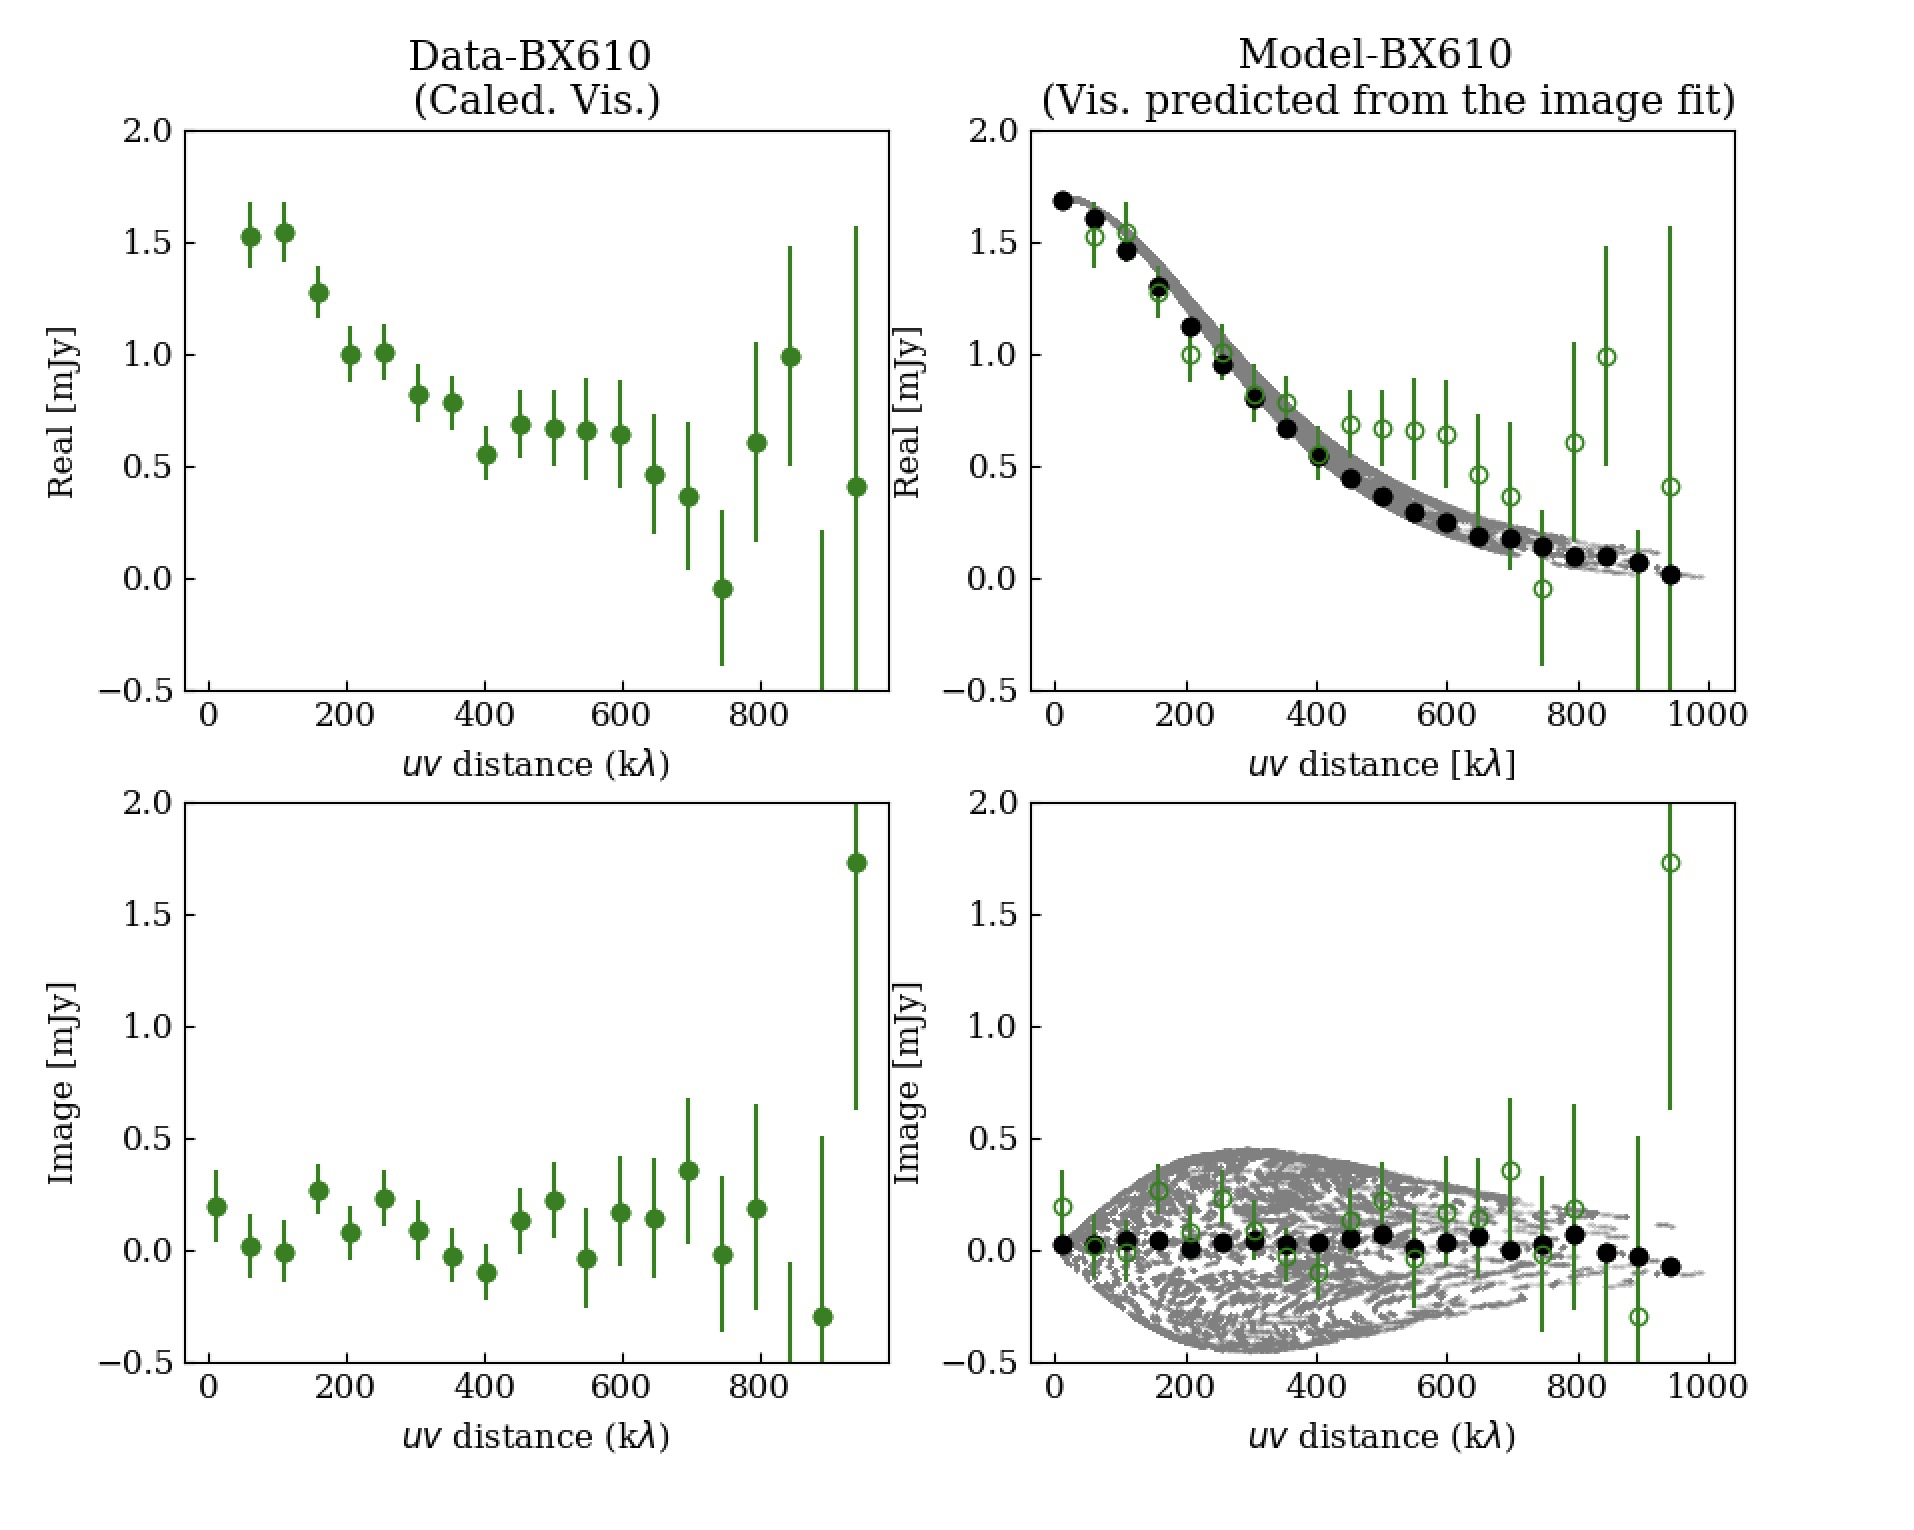
\includegraphics[width=0.48\textwidth]{figures/bx610-uvcont.png}
\caption{Highlight the advantage of searching for high spatial frequency information in UV.
}
\end{figure}

\begin{itemize}

\item no \clean\ 

\item no pixel gridding

\end{itemize}

deproject nearby galaxies to distant galaxies.

\subsection{Performance}

\subsubsection{Object/Line Decomposition}

\subsubsection{Source Extraction}


\section{Summary}

\clearpage











\appendix

\section{ALMA archival data of BX610}

\begin{deluxetable*}{ccccccrcccccc}%[htb!]
\tabletypesize{\small}
\tablecolumns{7} 
\tablecaption{ALMA Observations of BX610\label{tb:almaobs}}
\tablewidth{0pt} 
\tablehead{
%\multicolumn{1}{c}{Object}&
%\multicolumn{1}{c}{$\alpha_{\rm J2000}$}&
%\multicolumn{1}{c}{$\delta_{\rm J2000}$}&
%\multicolumn{1}{c}{$z$ }&
\multicolumn{1}{c}{Project Code}&
\multicolumn{1}{c}{P.I.} &
\multicolumn{1}{c}{Band} &
\multicolumn{1}{c}{Resolution} &
\multicolumn{1}{c}{LAS} &
\multicolumn{1}{c}{Lines} &
\multicolumn{1}{c}{$\Delta v$} &
\multicolumn{1}{c}{Cont.Freq.} &
\multicolumn{1}{c}{ToS}
%\multicolumn{1}{c}{}&
%\multicolumn{1}{c}{deg}&
%\multicolumn{1}{c}{deg}&
%\multicolumn{1}{c}{}&
%\multicolumn{1}{c}{}&
%\multicolumn{1}{c}{hr}&
%\multicolumn{1}{c}{} &
%\multicolumn{1}{c}{} &
%\multicolumn{1}{c}{}
}
\startdata
\toprule
%BX610		&356.5392 & 12.8221& 2.21	&
2013.1.00059.S	&Aravena, M.		&	4	& 0\farcs31	& 1\farcs63	&	\cofour/\cione	& 15.0\,\kms & 140GHz 	& 1.5\,hr	\\
2015.1.00250.S	&Aravena, M.		&	6	& 0\farcs25	& 1\farcs37	&	\coseven/\citwo & 18.5\,\kms & 233GHz	& 1.1\,hr	\\
2017.1.01045.S	&Brisbin, D. 		& 	4	& 0\farcs04	& 0\farcs57	&	\cofour/\cione	& 3.7\,\kms    &140GHz	& 3.9\,hr	\\
%VLA-D/11B-112		&Aravena	& 0\farcs25	&	\coone		& \citet{Aravena:2014aa}	\\
\bottomrule
\enddata
\tablecomments{
ToS: Time-on-Source, the aggregated integration time on the target field; Cont.Freq: the observed continuum frequency; LAS: largest angular scale, the maximal angular size of the spatial structure which the array configuration can observed; Resolution: the synthesized beam size reported in the ALMA archive imaging products.}
\end{deluxetable*}

We obtain the public ALMA data of BX610 from the ALMA Science Archive.
Three observations were carried out for the galaxy in 2013, 2015, and 2017 (see Table\,\ref{tb:almaobs}).
In all observation, four 1.875-GHz spectral windows were utilized for detecting line and continuum emission.
We rerun the ALMA pipeline calibration scripts supplied within the archival products for the raw visibility data using CASA \citep{McMullin:2007ta}. 
This generated the fully calibrated visibility, and we performed additional manual inspection to flag bad data from a small number of antenna/channel by their abnormal amplitude.

While our program can model data in the $uv$ domain, we have imaged the visibility data and model for testing on the image-domain modeling capability as well as quality inspection/visualization.
For all imaging, we produce data cubes using the Briggs ROBUST weighting of $R=0.5$ and the synthesized beams are sampled by at least nine pixels.


In four 1.875-GHz spectral windows, we tuned two of them for detecting continuum emission at 105.1GHz, with the other two centered around 92.2 and 94.0\,GHz. 
The later two windows were targeted to the \cothree\ emission from two different redshifts ($z=2.67$ and $2.75$), which are associated with the SMG and a QSO system previously identified in optical spectra.
The channel width of all four spectral windows was set to 7.8125\,MHz, which is equivalent to a velocity resolution of $22.5-25.5$\,km/s.

We calibrated the visibility data using the ALMA pipeline implemented within CASA\,ver.\,5.4.0.
We imaged two separate spectral cubes from two line windows, one continuum image from two continuum windows.
The imaging pixel was set to 0\farcs2, and we adopted an imaging channel width of three times that intrinsic visibility channel, which provides a resolution of $\sim$75\,km/s for the CO 3-2 line at the expected SMG redshift.

With a robust weighting of $R=1$, the final imaging achieves a spatial resolution of $\sim1\farcs5\times1\farcs2$ in the \cothree\ window. The sensitivity of the continuum image reaches 6.7\,uJy/beam, with the line channel sensitivity archive 0.1\,mJy/beam.
We didn't perform continuum subtraction in the visibility data and instead to choose image-domain subtraction for any identified line emitter on an individual basis.



\section{SINFONI observations of BX610}

\section{Example of Input Files}

The program will save the results into the a parameter file which contain the best-fit resultsg same parameter file
\begin{figure}%[h!]
\centering
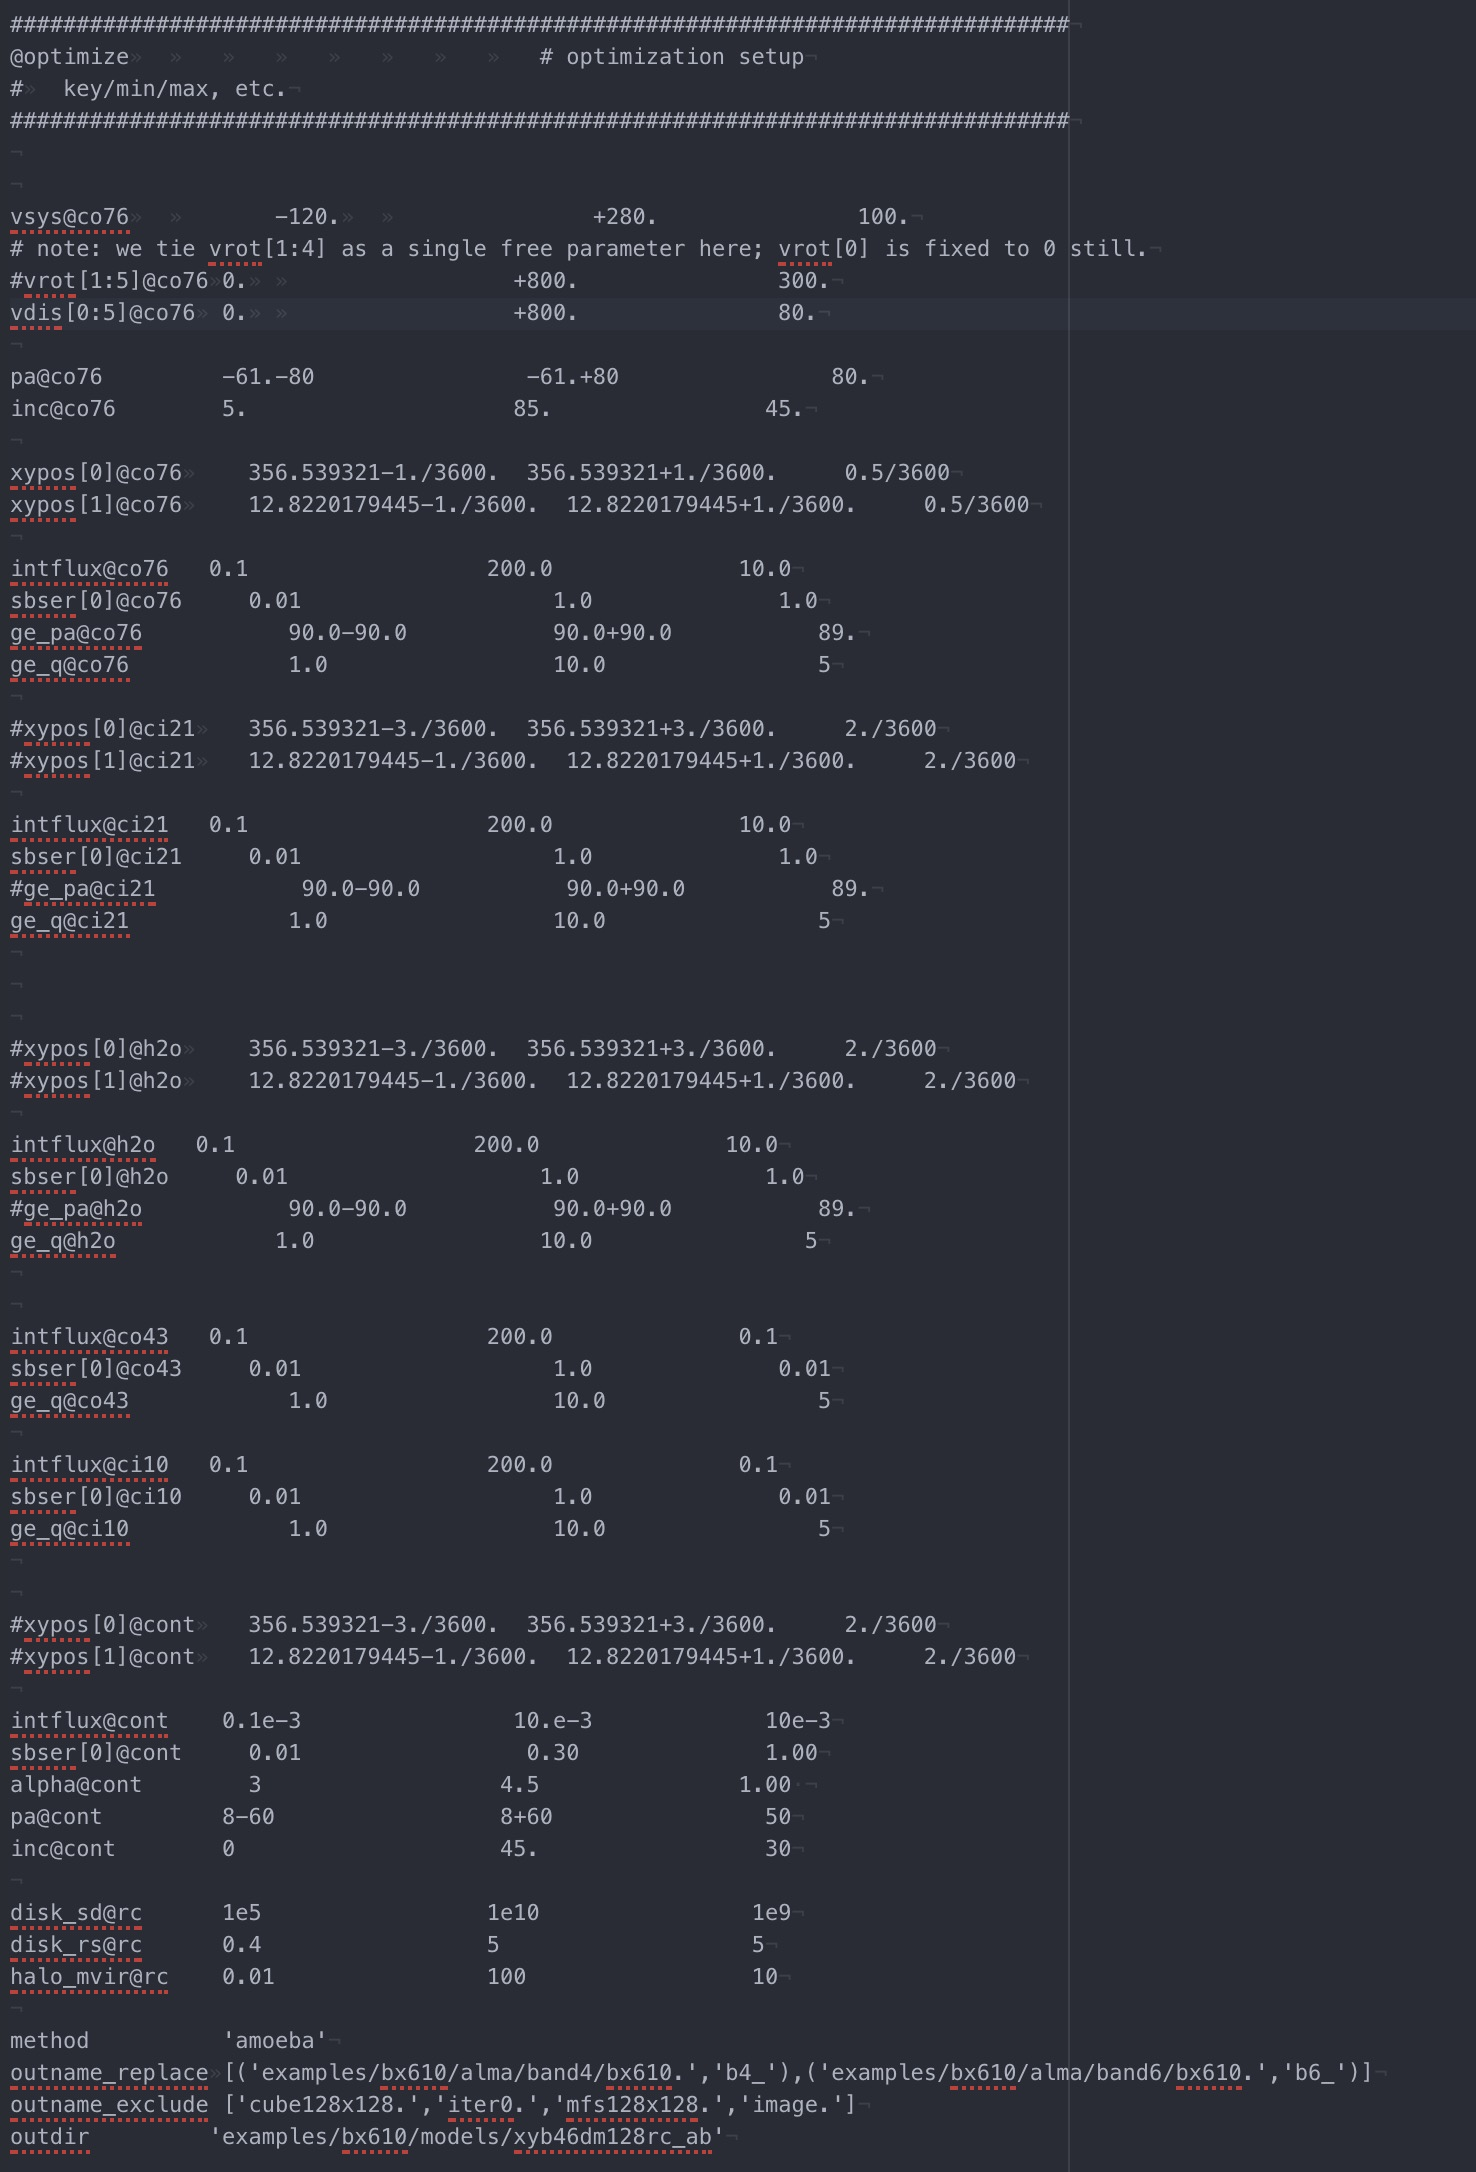
\includegraphics[width=0.48\textwidth]{figures/example-inp.jpeg}
\caption{Highlight the advantage of searching for high spatial frequency information in UV.
}
\end{figure}


\section{Comparison Summary}


\begin{deluxetable*}{cccrccccccccc}[htb!]
\tabletypesize{\small}
\tablecolumns{7} 
\tablecaption{Summary \label{tb:sample}}
\tablewidth{0pt} 
\tablehead{
\multicolumn{1}{c}{Name}&
\multicolumn{1}{c}{Reference} &
\multicolumn{1}{c}{Type} &
\multicolumn{1}{c}{DataType}&
\multicolumn{1}{c}{Platform/Lang.}&
\multicolumn{1}{c}{Fitting}&
\multicolumn{1}{c}{Availability}
}
\startdata
\toprule
\multicolumn{7}{c}{2D (velocity-field) Kinematics Fitting}\\
\midrule
ROTUR	&	\cite{van-Albada:1985aa}	&	Tiled-ring	&	SpectralCube &  GIPSY\tablenotemark{1}		& lmfit	& S/B \\
\midrule
\multicolumn{7}{c}{3D Kinematics Modeling}\\
\midrule
\galmod		&	\cite{van-der-Hulst:1992aa}			&	Tiled-ring	&	SpectralCube	& lmfit	& GIPSY					& S/B \\
KinMS		&	 \citep{Davis:2013aa}	&	Tiled-ring	&	SpectralCube	& lmfit	& IDL/Python\tablenotemark{2}				& S/B \\
\midrule
\multicolumn{7}{c}{3D (spectral-cube) Kinematics Fitting}\\
\midrule
\tirific		&	\cite{Jozsa:2007aa}		&	Tiled-ring		&	SpectralCube	& lmfit  	& CASA				& S/B \\
\barolo	& 	\cite{Di-Teodoro:2015aa}	&	Tiled-ring		&	SpectralCube	& lmfit	& C++				& S/B \\
\galpak	&	\cite{Bouche:2015aa}			&	Tiled-ring		&	SpectralCube	& lmfit	& C++				& S/B \\
\midrule
\multicolumn{7}{c}{2D Morhology Fitting}\\
\midrule
GALFIT	\\
PHOTUTILS \\
SEXTRACTOR \\
\bottomrule
\enddata
\tablecomments{Modeling and Fitting, not every program provide the fitting function.
Many programs also include source detection propurse but this is not one of them,
}
\tablenotetext{1}{The same algorithm is built-into NEMO/AIPS}
\tablenotetext{2}{A modified Python-version of KinMS is implemented in \gmake\ for generating intrinsic models in the form of spectral cubes}
\end{deluxetable*}

\section{keywords}


\begin{deluxetable*}{lll}[htb!]
\tabletypesize{}
\tablecolumns{7} 
\tablecaption{Examples of Different Rotational Curve Forms \label{tb:rc_examples}}
\tablewidth{0pt} 
\tablehead{
\multicolumn{1}{l}{Type}&
\multicolumn{1}{l}{Description} &
\multicolumn{1}{l}{Keyword}
}
\startdata
\toprule
Table		&	A cubic spline interpolated from a rotation curve table 		& vrot = [$v_{\rm rot,1}$, $v_{\rm rot,2}$, ...] \\
			&													& vrad = [$r_{\rm 1}$, $r_{\rm 2}$, ...] \\
\midrule
Analytical		&	an analytical form specified by a math expression 	& vrot = (math\_expr, p1, p2, ...)\\
\cmidrule{2-3}				
			&	a piece-wise RC: $v_{\rm rot}$ linearly increases to $v_{\rm max}$ 		& vrot = (`minimum(vrad/p2,1)$*$p1', $v_{\rm flat}$, $r_{\rm t}$)	\\
			& 	``arctan'': $v(r)=v_{\rm max}\frac{2}{\pi}\arctan(r/r_{\rm t})$ 	&	vrot = (`p1$*$2/pi$*$arctan(vrad/p2)', $v_{\rm max}$, $r_{\rm t}$) \\
			&													&	alt. vrot = (`arctan', $v_{\rm max}$, $r_{\rm t}$) \\
			&	``exp'': $v(r)=v_{\rm max}[1-\exp(-r/r_{\rm t})]$			&	vrot = (`p1$*$(1-exp(-vrad/p2))', $v_{\rm max}$, $r_{\rm t}$) 	\\
			&													&	alt. vrot = (`exp', $v_{\rm max}$, $r_{\rm t}$) 	\\
			&	``tanh'': $v(r)=v_{\rm max}\tanh(r/r_{\rm t})$				&	vrot = (`p1$*$tanh(vrad/p2)', $v_{\rm max}$, $r_{\rm t}$) 	\\
			&													&	alt. vrot = (`tanh', $v_{\rm max}$, $r_{\rm t}$)	\\				
\midrule
Dynamics		&	derived from a gravitational potential model 				&	vrot = (`dynamics', model\_name)	\\	
\bottomrule
\enddata
%\tablecomments{}
%\tablenotetext{1}{The same algorithm is built-into NEMO/AIPS}
\end{deluxetable*}


\section{Diagnostic Plots}

Observational data are acquired at most in three dimensions ($x$-$y$-freq/wavelength).
We therefore divided our diagnostic plots into three groups, depending on the number of dimension in which they are presented.
Various diagnostic plots can be produced by choosing different dimension combinations and adjusting restribuctions of subregions in which the data are extracted.

1D plots -- intensity vs. spectral dimension
This is just the display of spectra extracted at various aperture
\begin{figure*}%[h!]
\centering
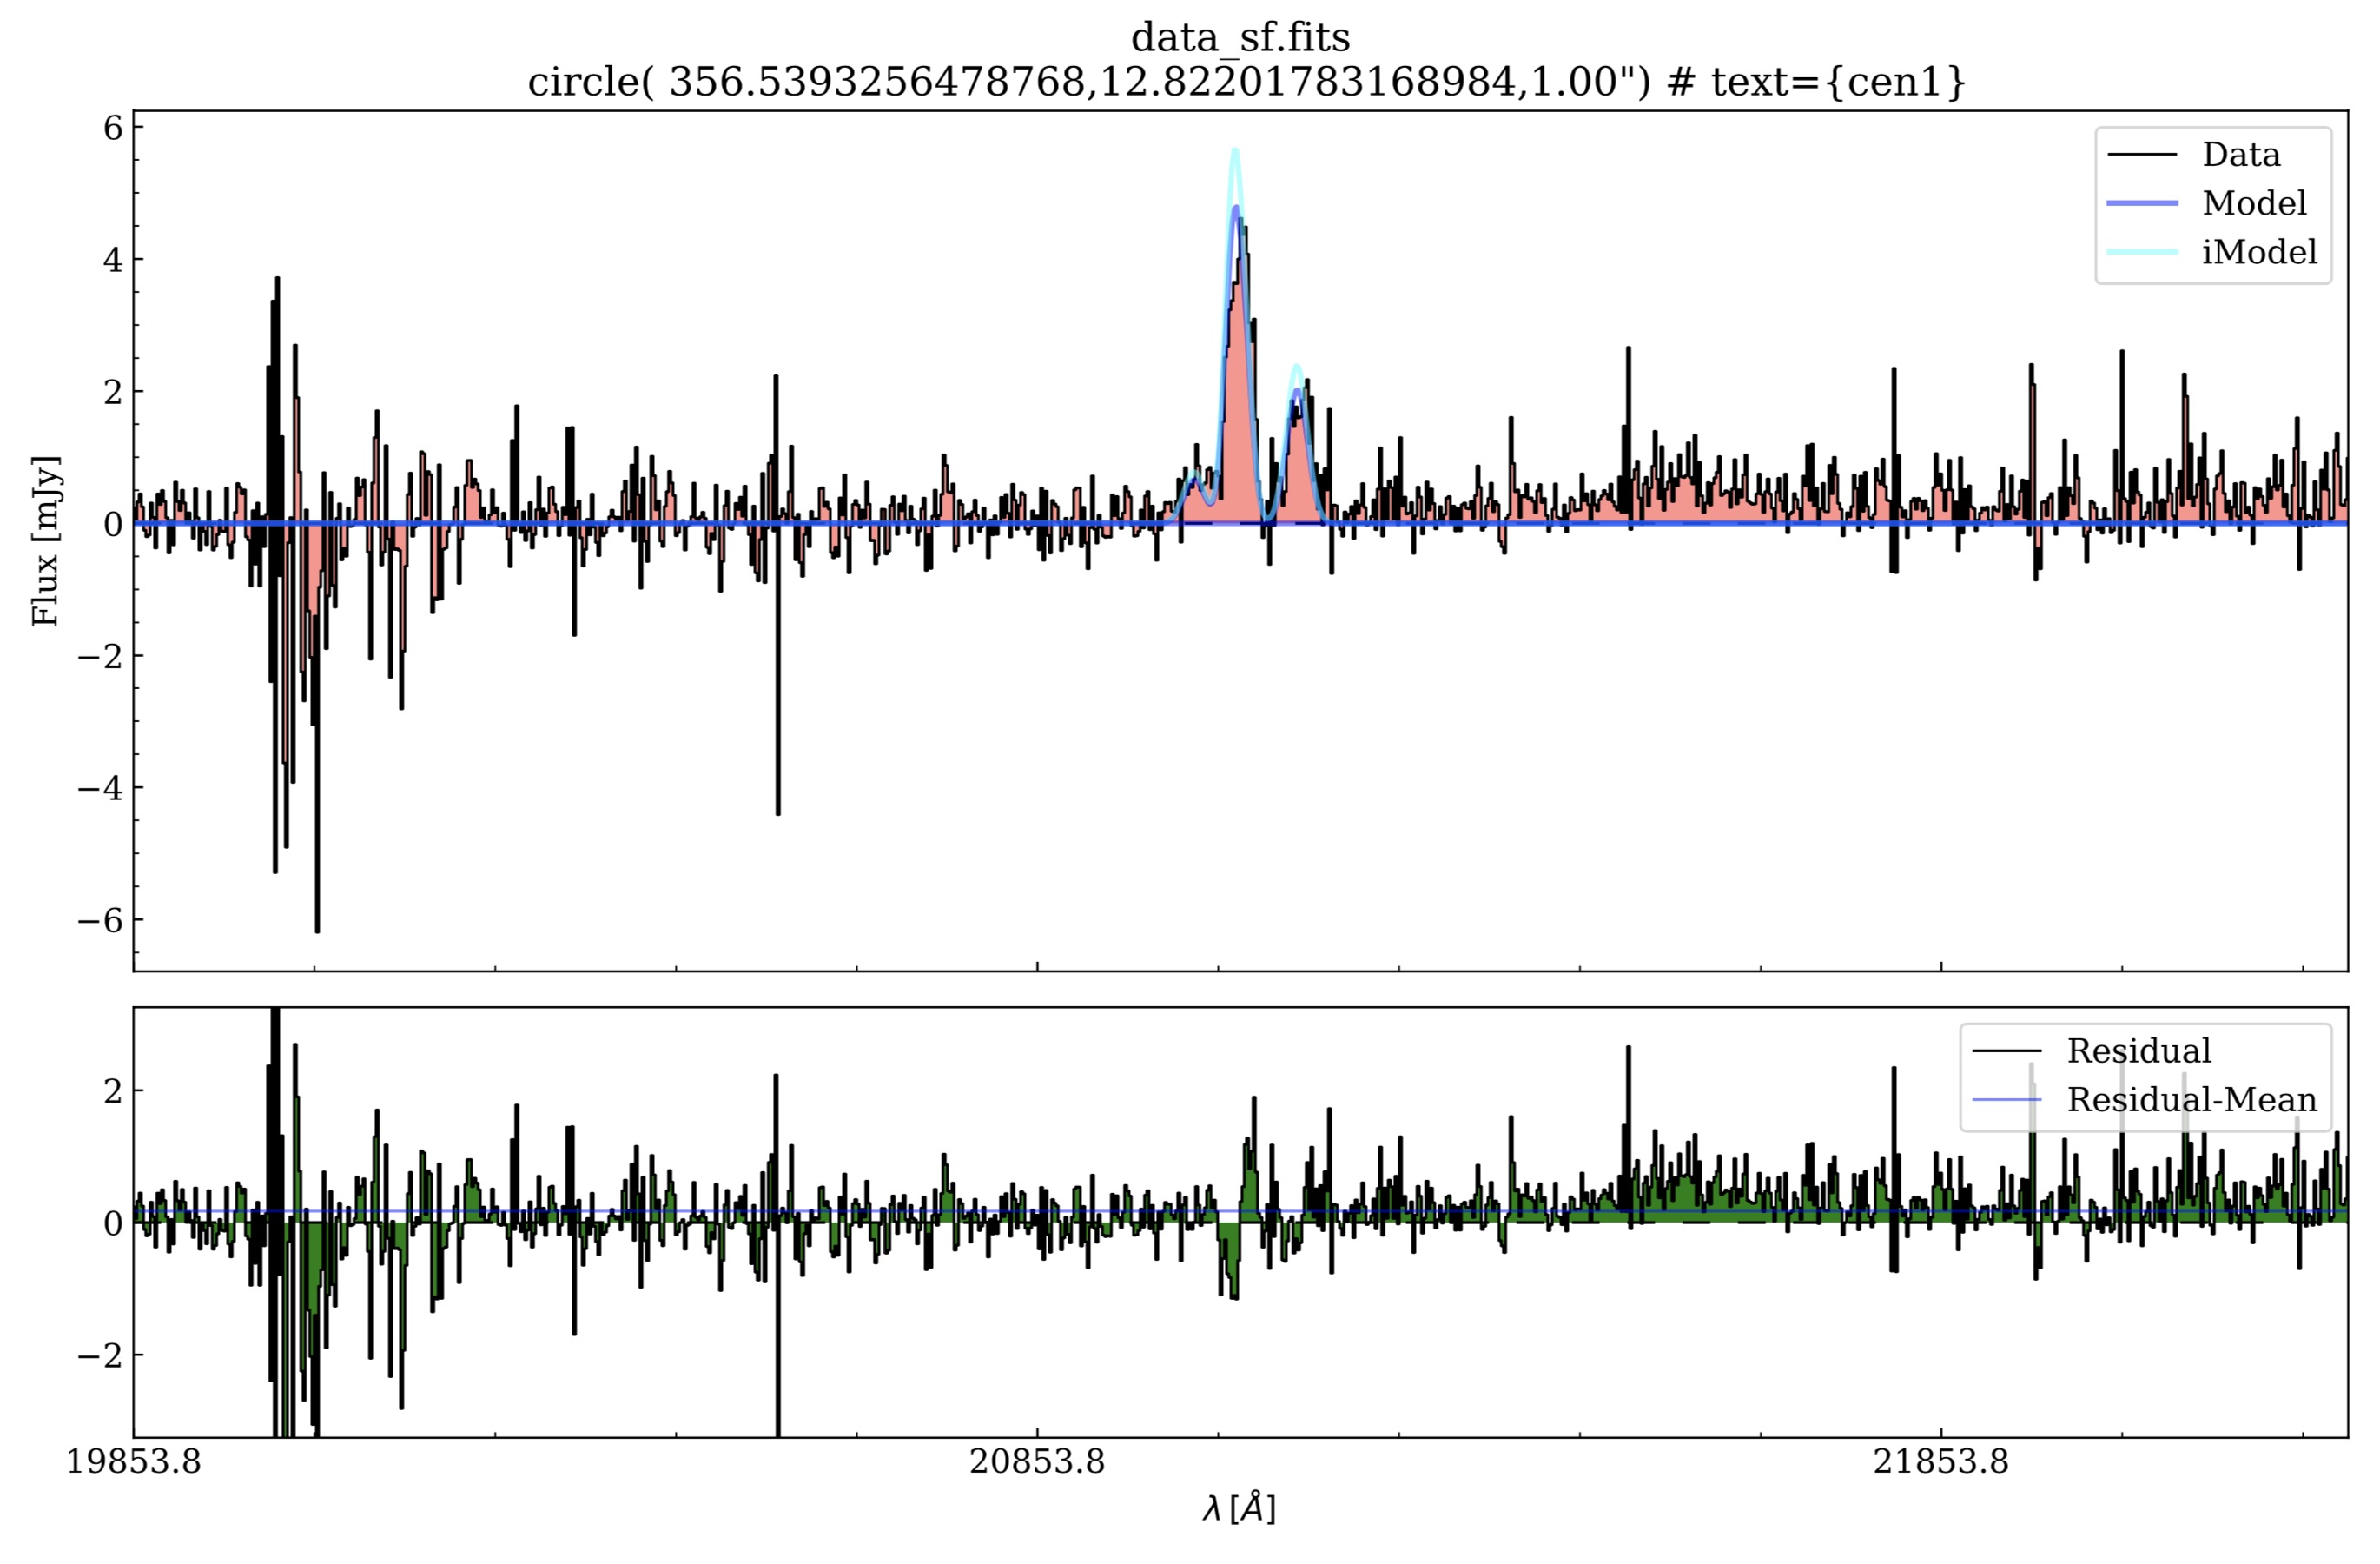
\includegraphics[width=0.40\textwidth]{figures/bx610-sinfoni-spec.jpeg}
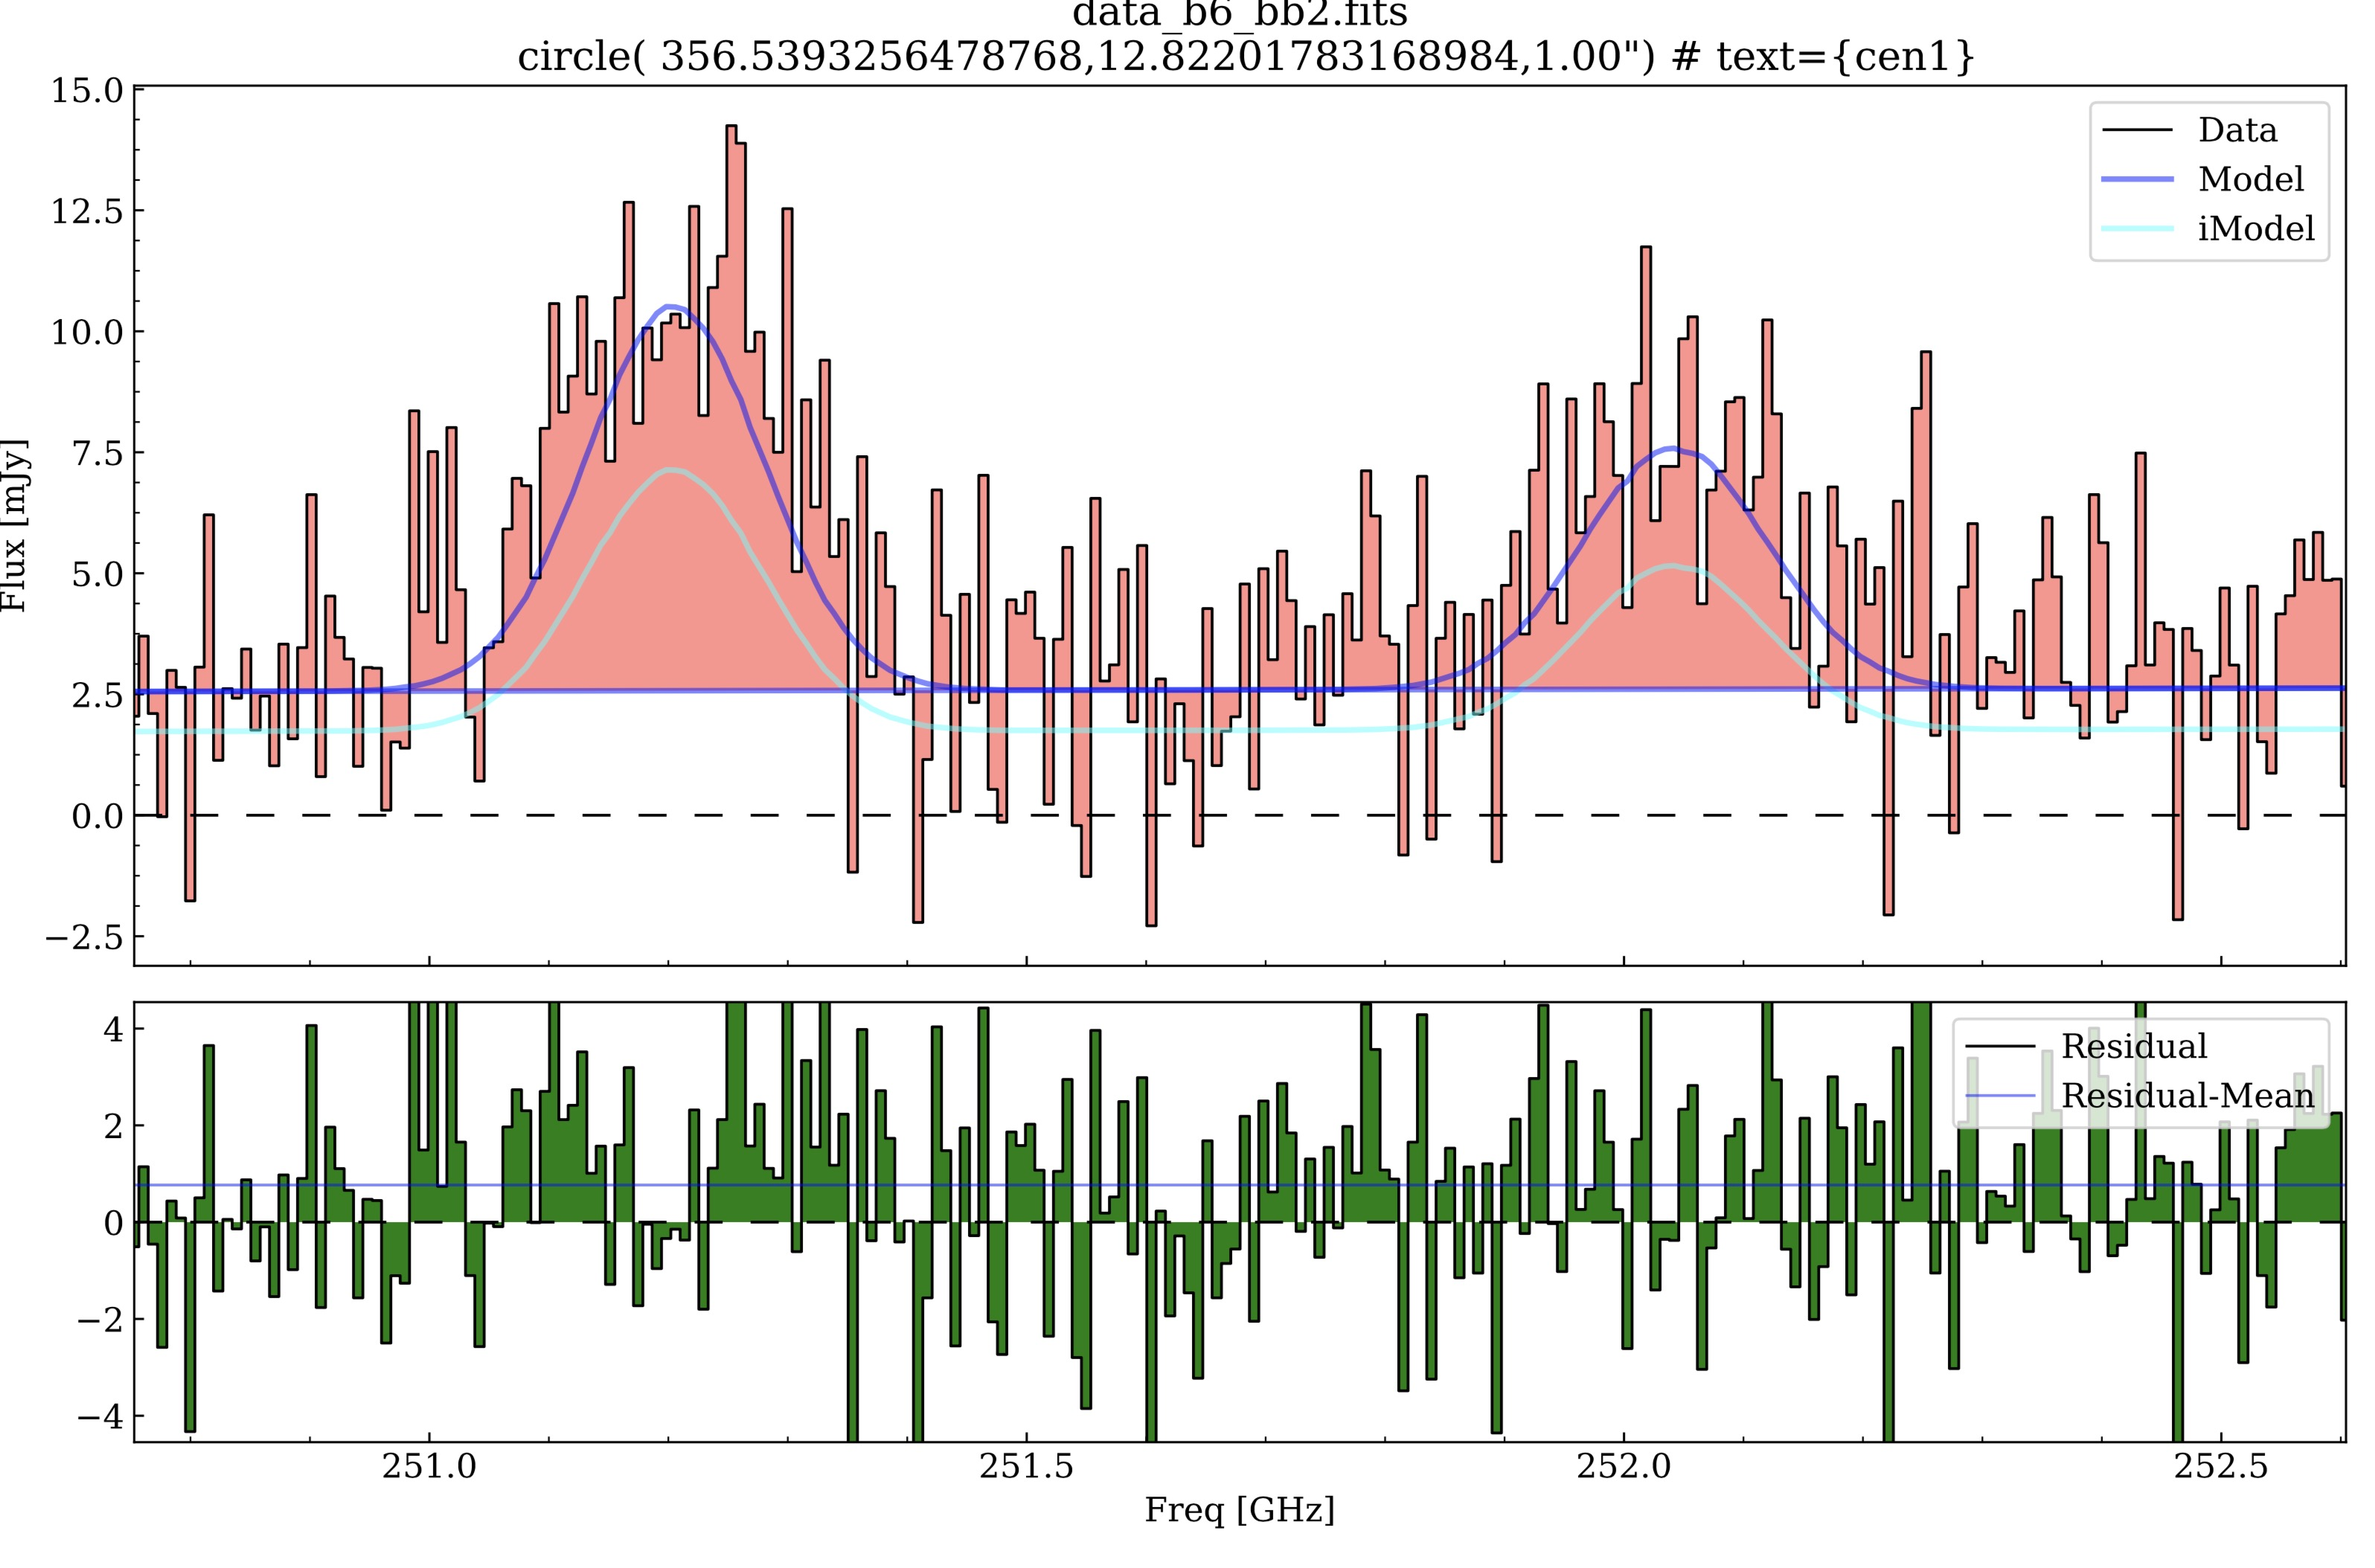
\includegraphics[width=0.40\textwidth]{figures/bx610-alma-spec.jpeg}
\caption{Highlight the advantage of searching for high spatial frequency information in UV.
}
\end{figure*}

1D plots -- intensity vs. spatial dimension
This is the display of radial profile (deprojected) or intensity profile along a spatial slice. or along major minor axis.
\begin{figure*}%[h!]
\centering
\includegraphics[width=0.48\textwidth]{figures/hi_radprofile.jpg}
\caption{1D diagnostic plots. Intensity vs. spatial: SB radial profile (after deprojection), Highlight the advantage of searching for high spatial frequency information in UV.
}
\end{figure*}

1D plots -- display of physical properties (for example, radial vs. rotational velocity / dispersion)
\begin{figure}%[h!]
\centering
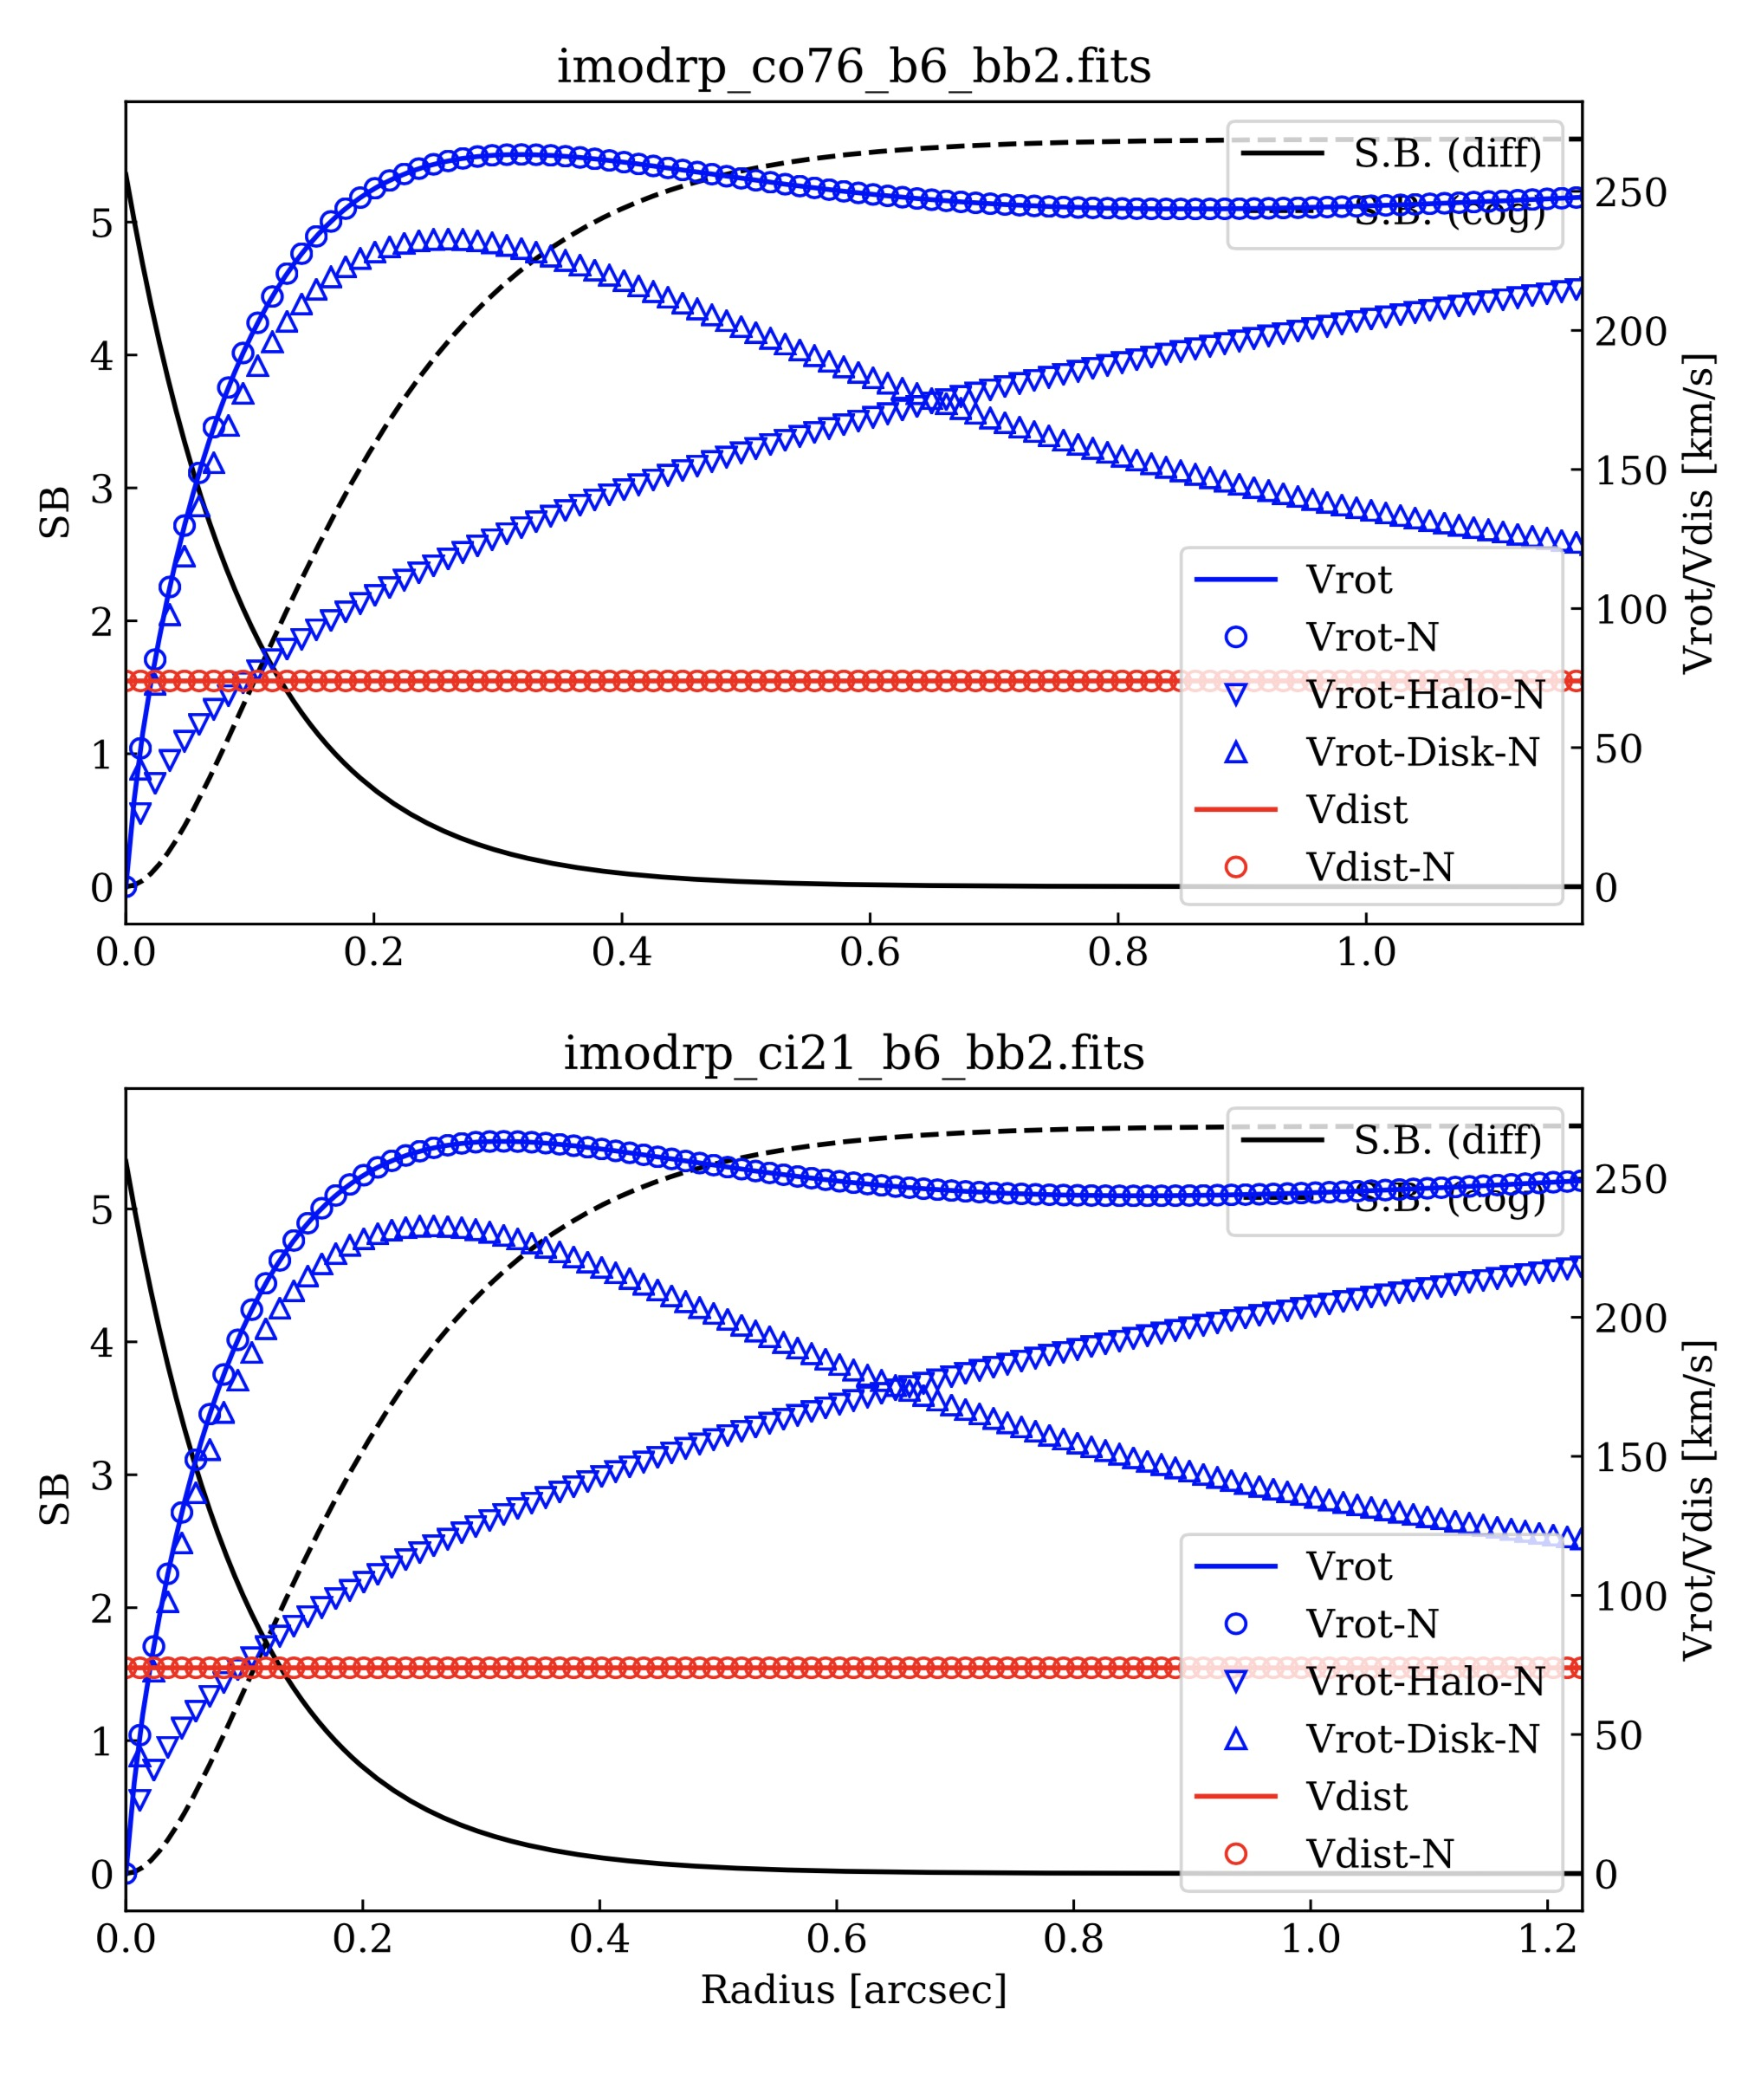
\includegraphics[width=0.48\textwidth]{figures/bx610-alma-rc.jpeg}
\caption{1D diagnostic plots. Intensity vs. spatial: SB radial profile (after deprojection), Highlight the advantage of searching for high spatial frequency information in UV.
}
\end{figure}

2D plots -- intensity / velocity centroid / velocity dispersion  vs. x-y
These two-dimensional representation show the spatial distribution of various physical properties extracted from the data: for example, the integrated intensity, spectral line centroid, line widths (typically referred to as moment-0/1/2 images).
The first (veolocity field) and second (velocity dispersion) moments images of a spectral cube can help reaveal galaxies kinematic details. However, the a 2D velocity field / dispersion collapsed the 3D PPV structure into  is a limited representation of the intrisnic gas kinmetics within a galaxy due to observational effect such as low S/N or beam smearing, and the result may depend on extraction methods.

 but all of them are subjected to the extraction methods and bserevational effect (low S/N, beam smearing).
If we restrict the data into a small spectral range, then we can create a channel maps
\begin{figure}%[h!]
\centering
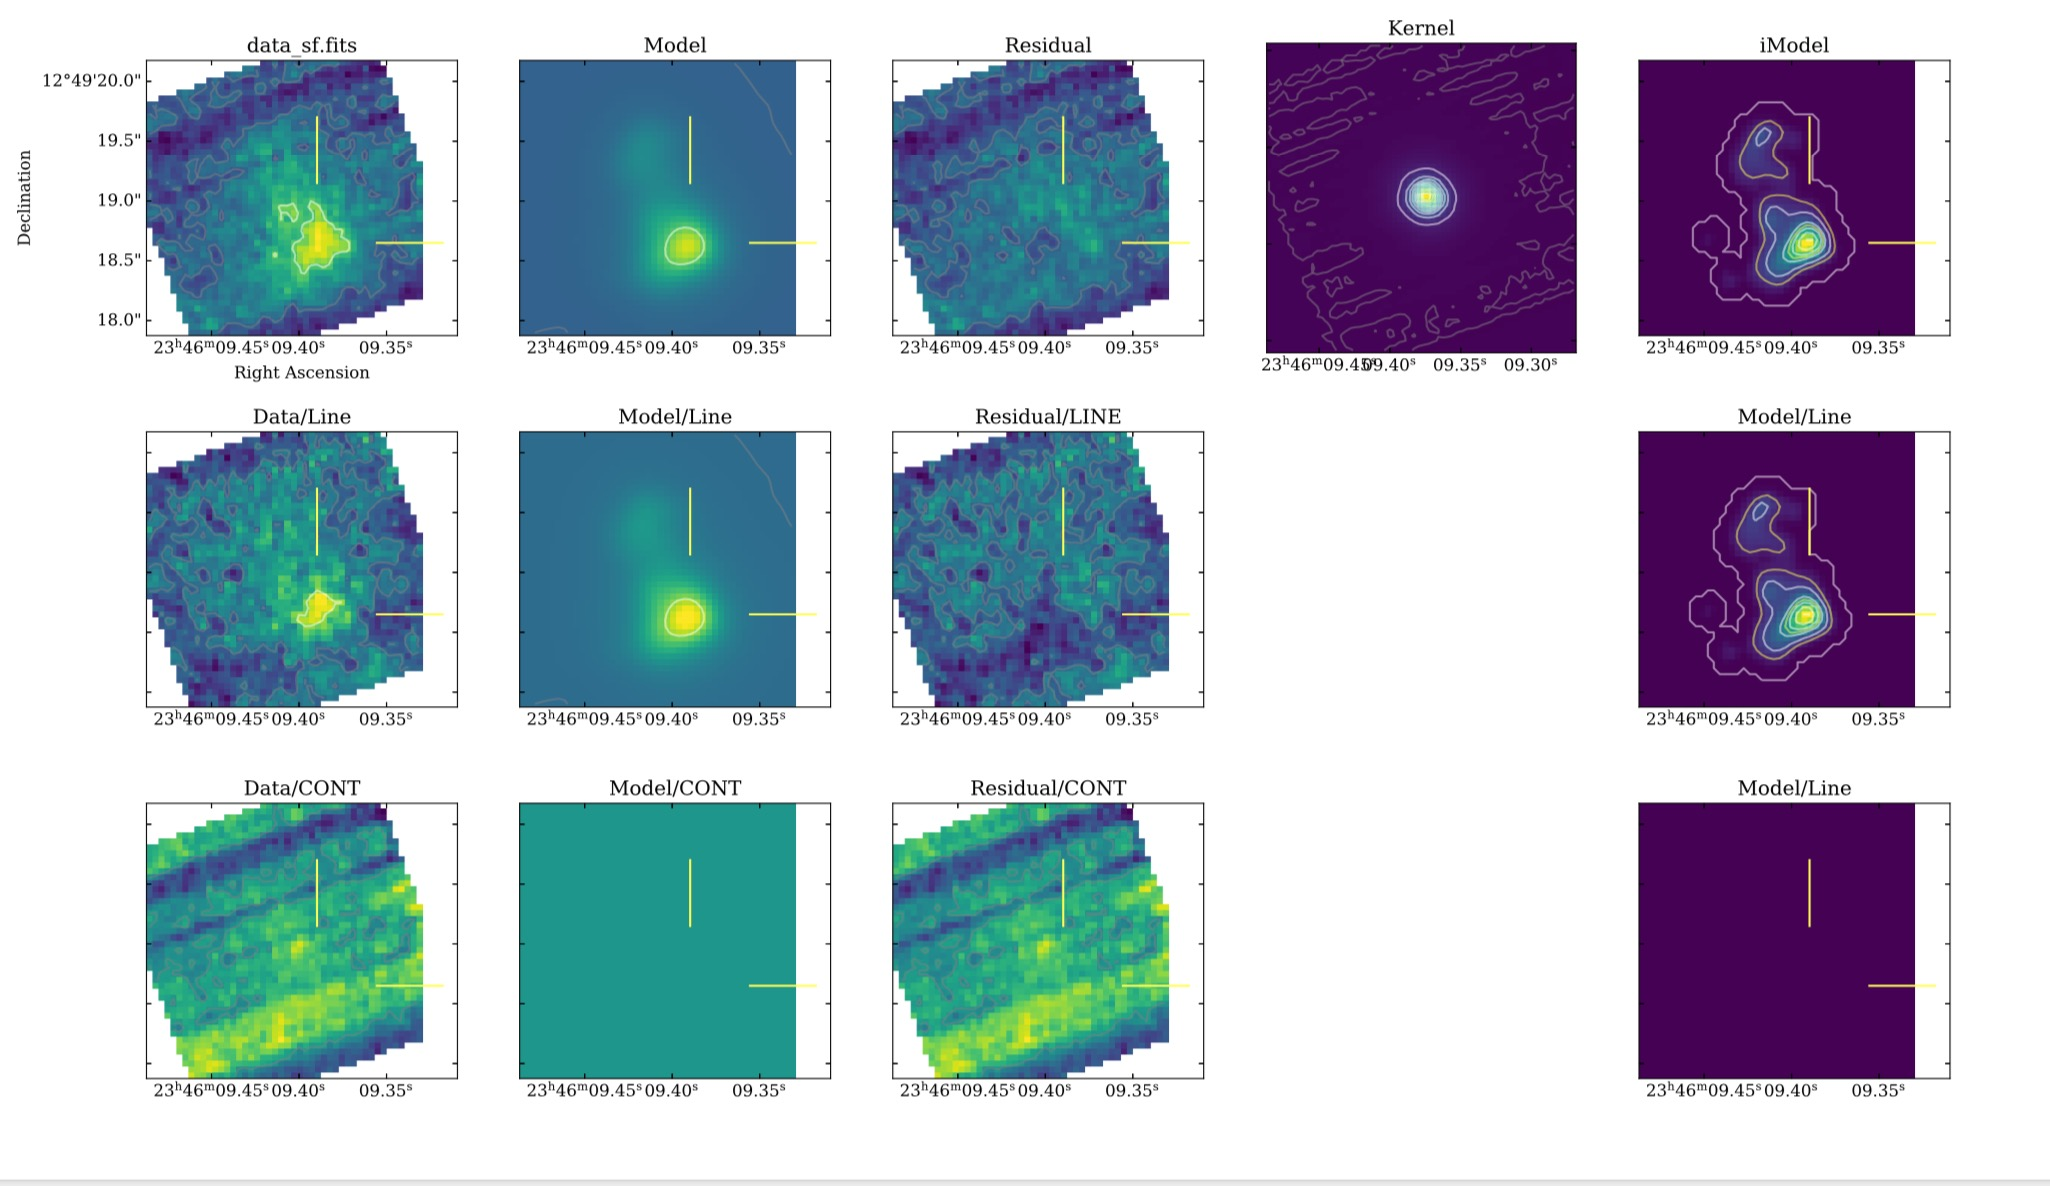
\includegraphics[width=0.48\textwidth]{figures/bx610-sinfoni-xy.jpeg}
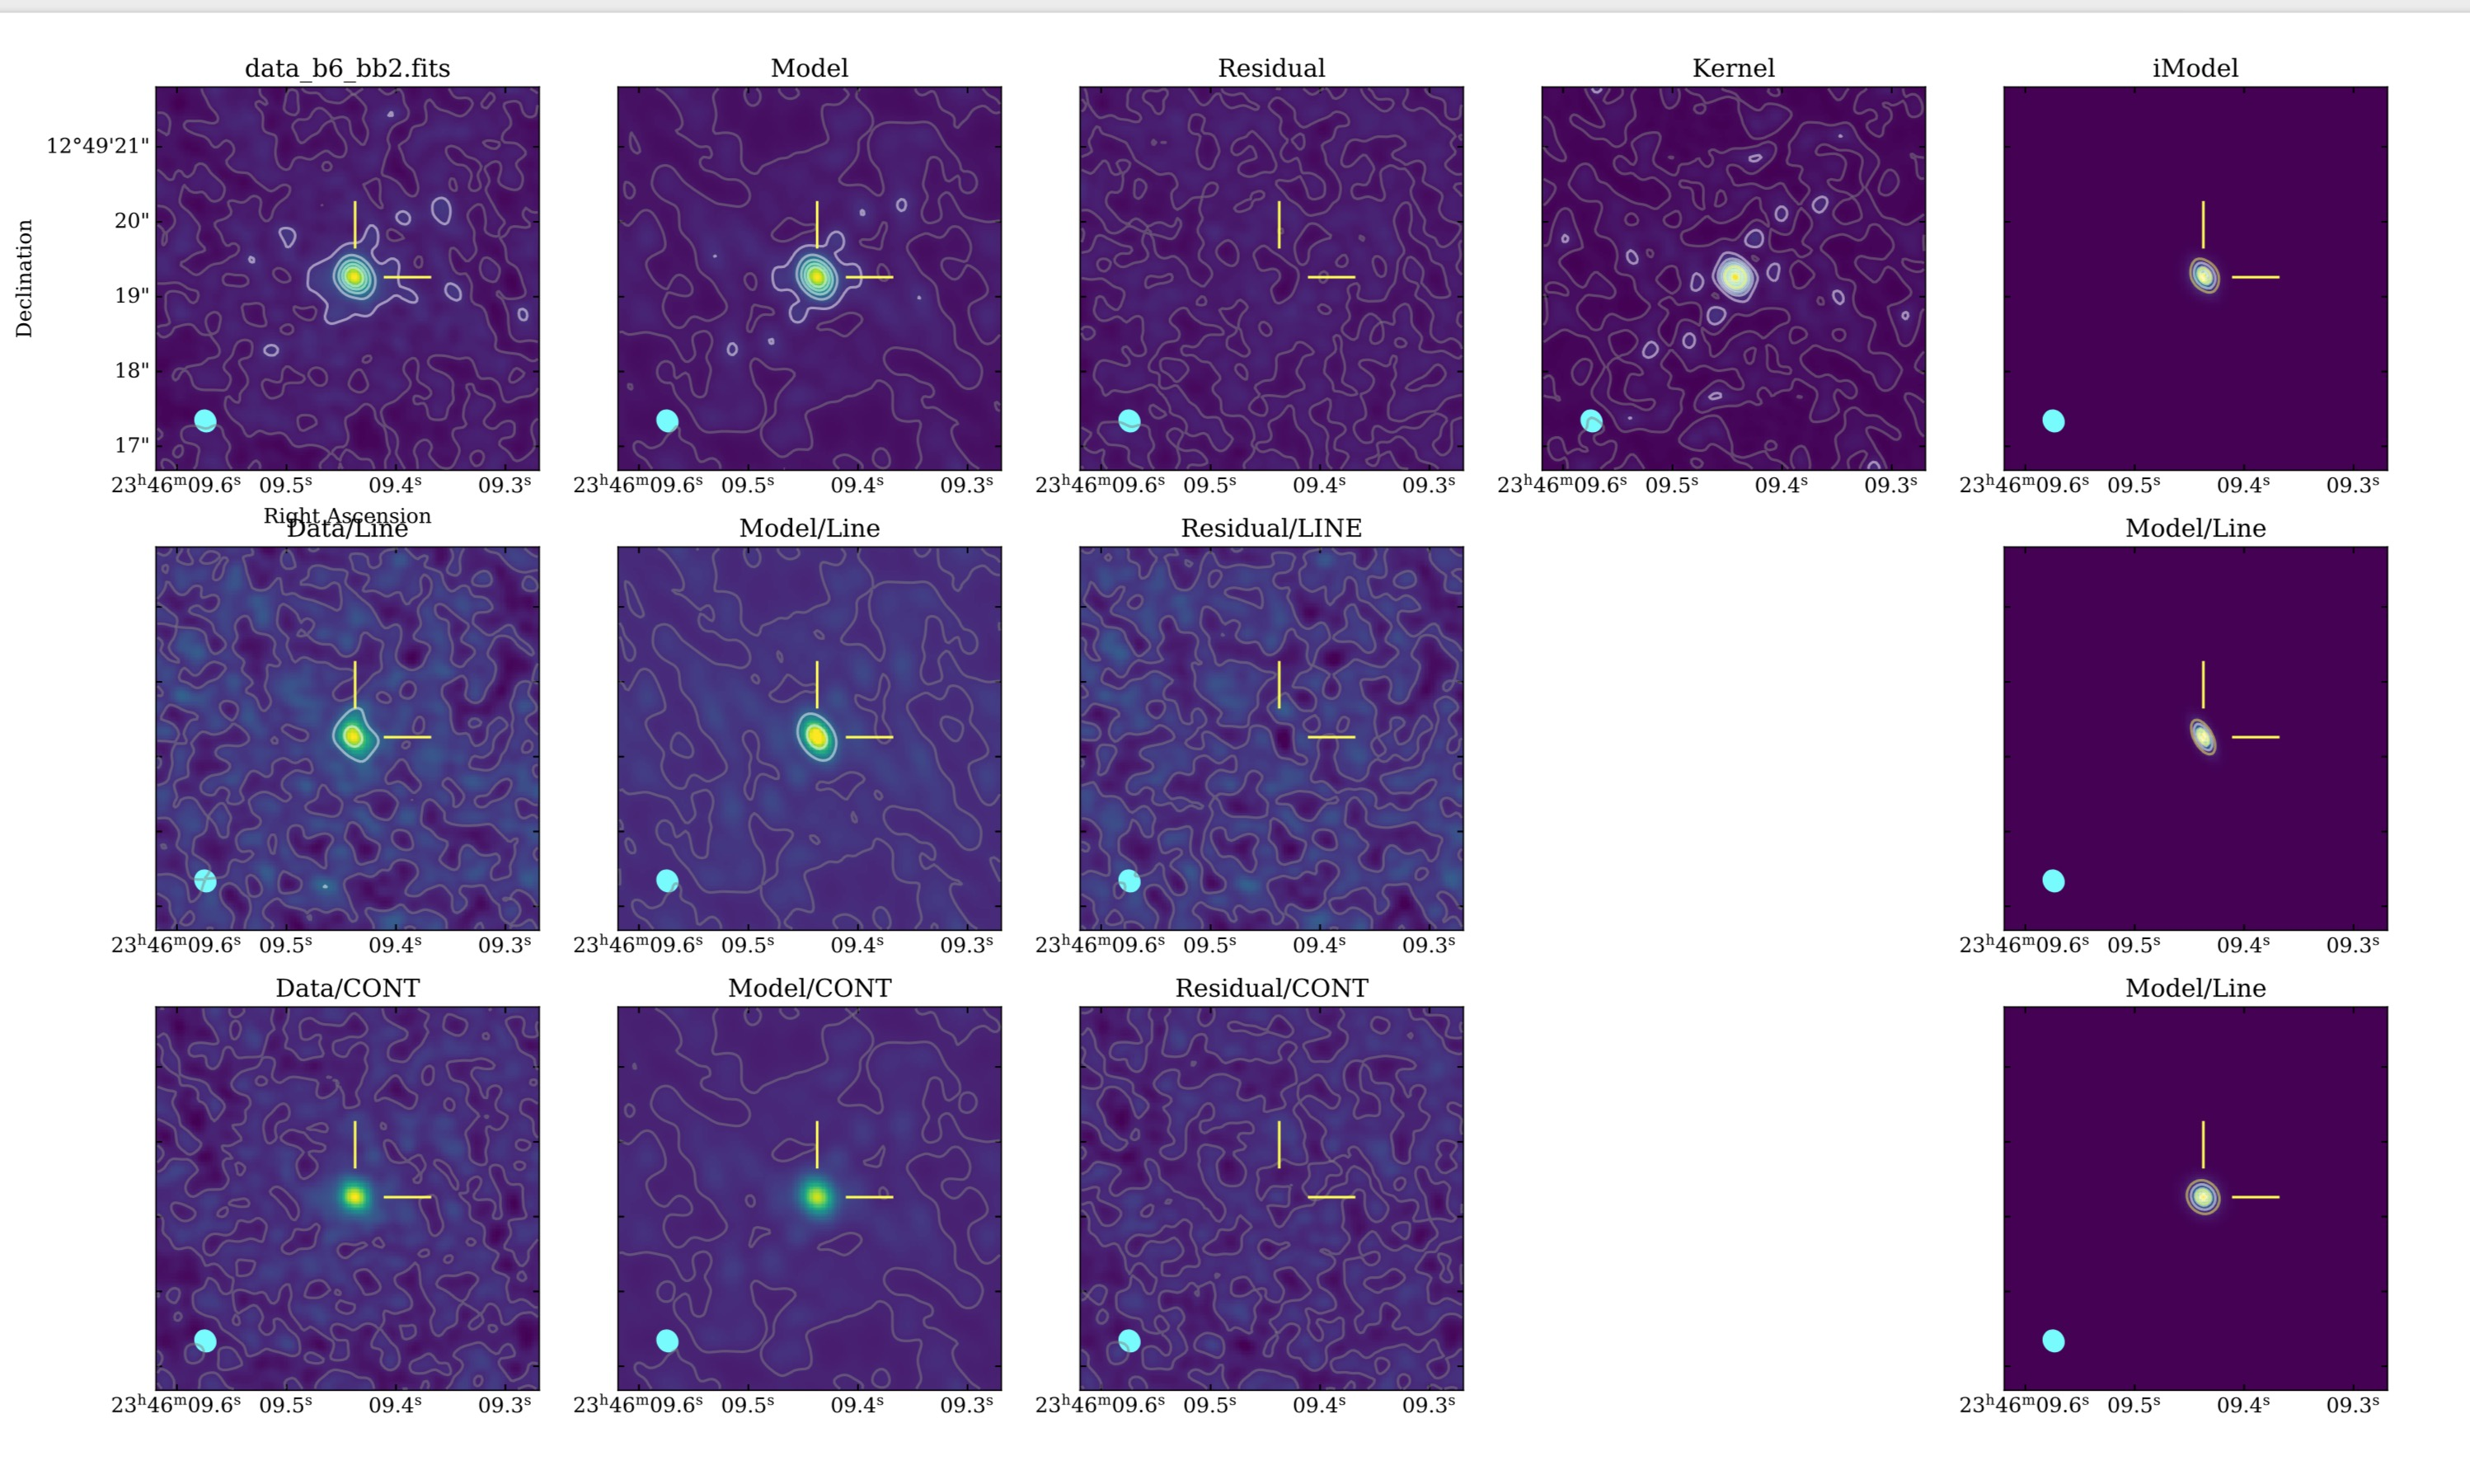
\includegraphics[width=0.48\textwidth]{figures/bx610-alma-xy.jpeg}
\includegraphics[width=0.48\textwidth]{figures/example_xy.jpg}
\includegraphics[width=0.48\textwidth]{figures/example_channel.jpg}
\caption{Highlight the advantage of searching for high spatial frequency information in UV.
}
\end{figure}


2D plots -- intensity / velocity centroid / velocity dispersion  vs. r-freq/wavelength

\begin{figure}%[h!]
\centering
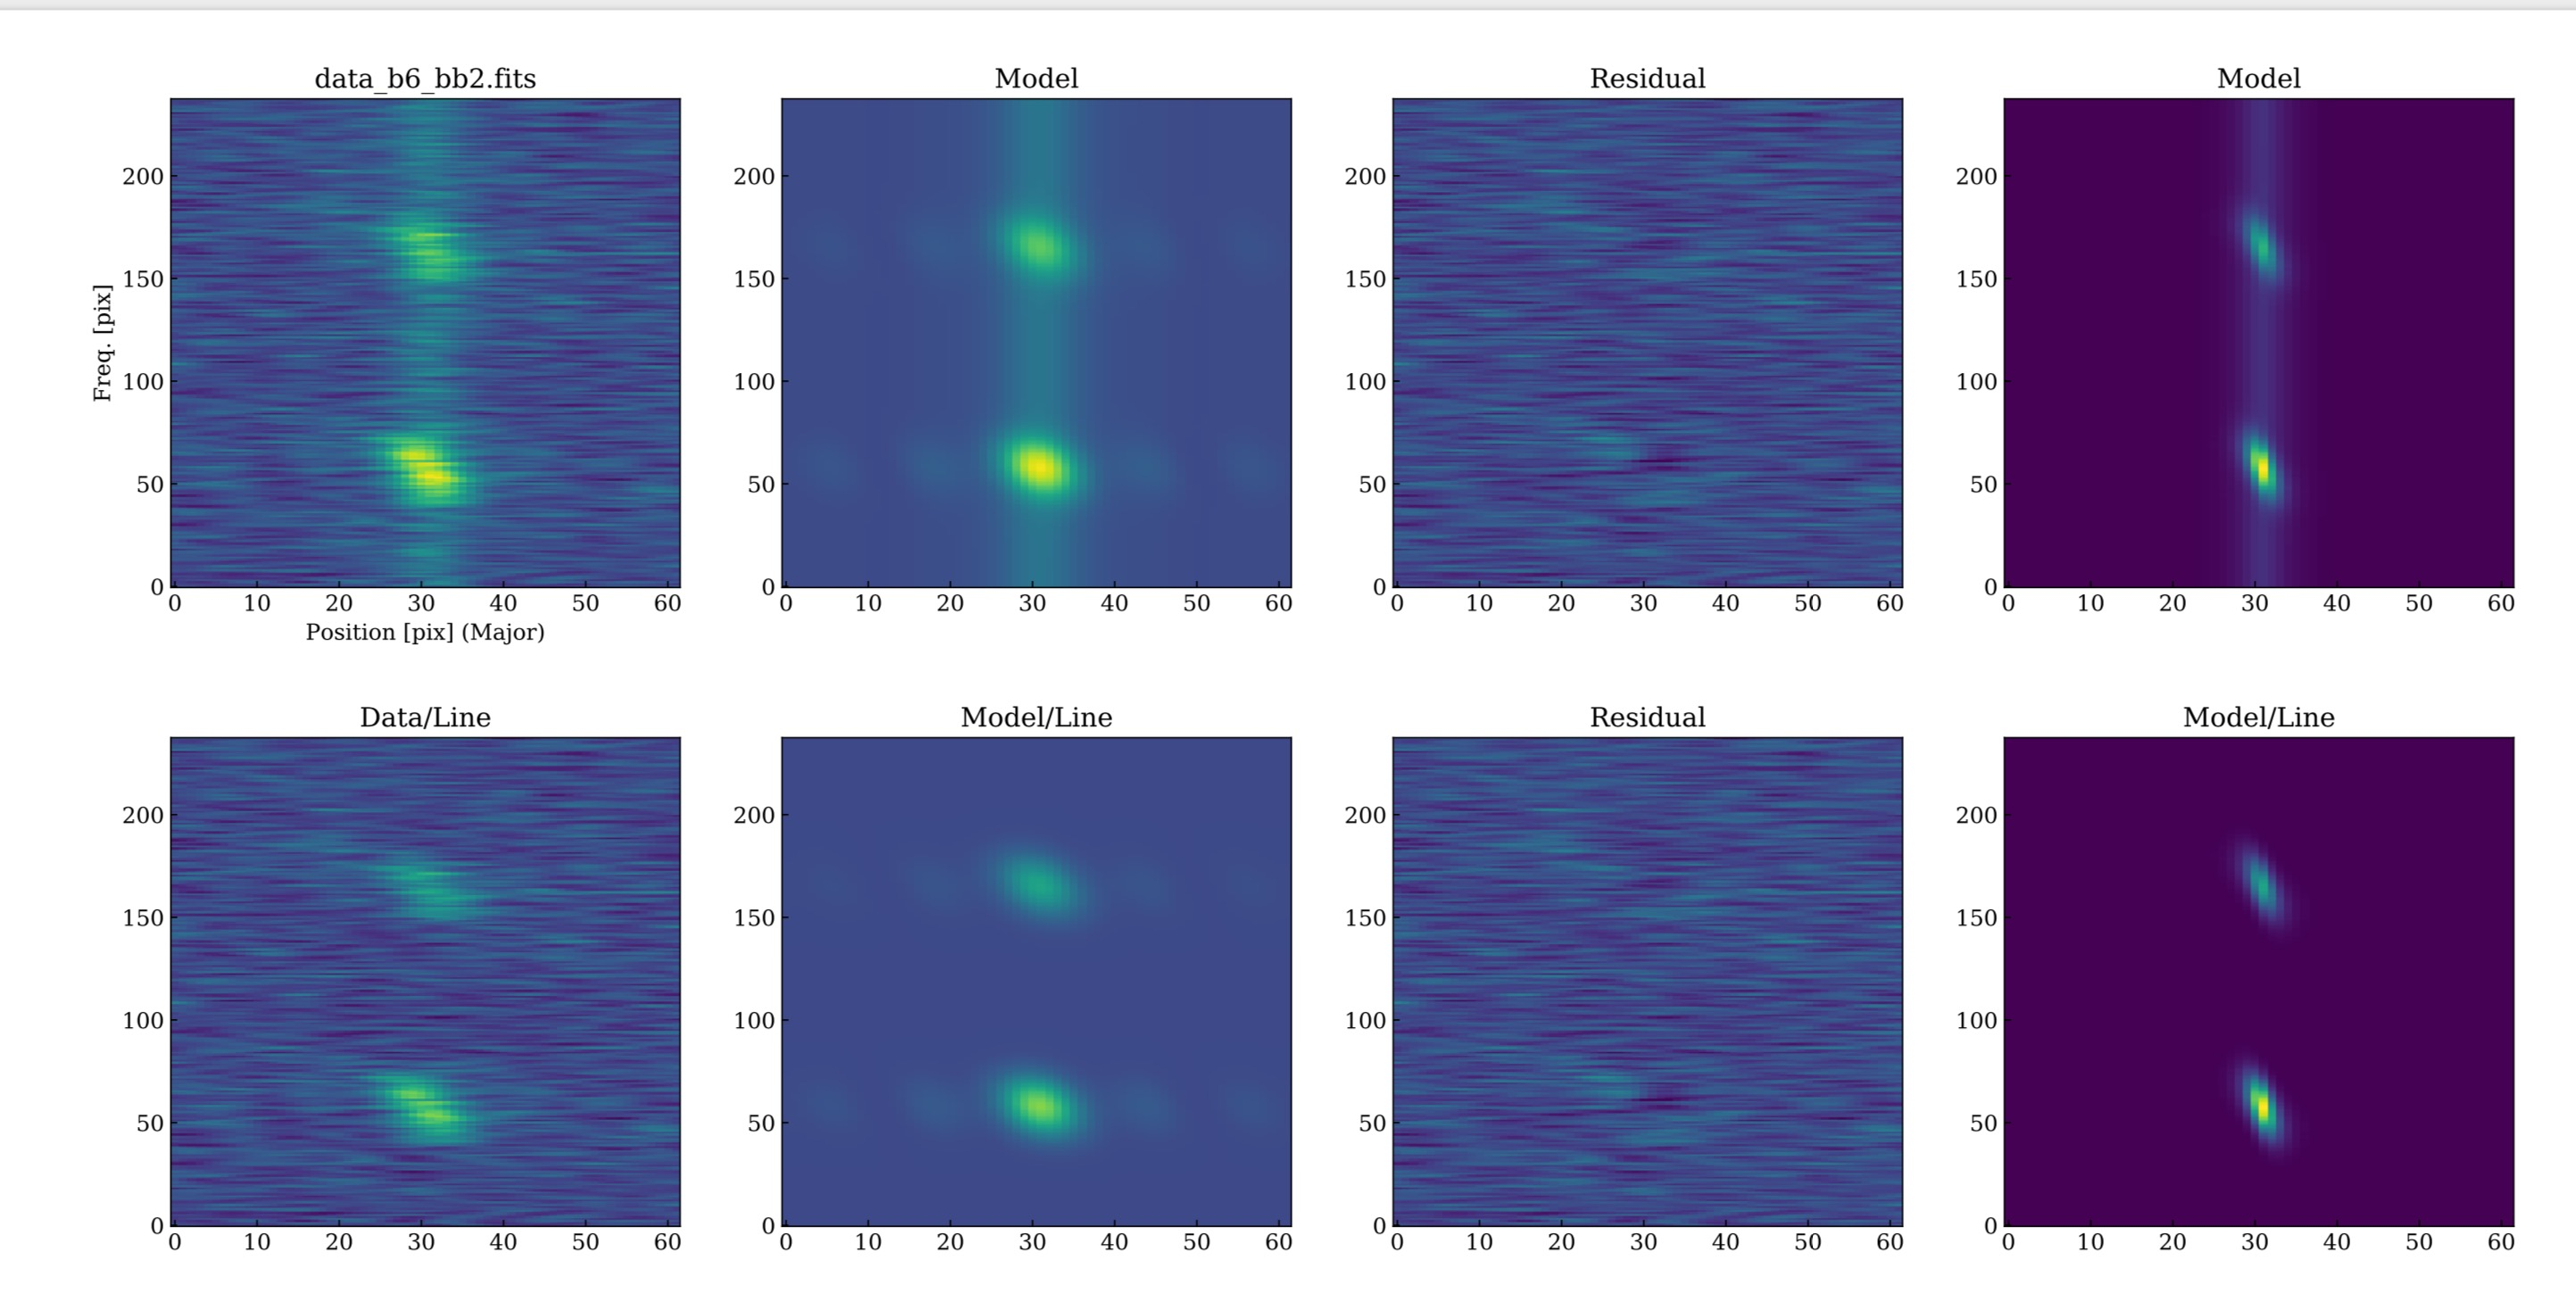
\includegraphics[width=0.48\textwidth]{figures/bx610-alma-pv.jpeg}
\includegraphics[width=0.48\textwidth]{figures/example_pv.jpg}
\caption{1D diagnostic plots. Intensity vs. spatial: SB radial profile (after deprojection), Highlight the advantage of searching for high spatial frequency information in UV.
}
\end{figure}

3D plots -- rendering
% https://blog.kitware.com/introducing-slicerastro-a-visualization-tool-for-hydrogen-in-galaxies/

%\begin{figure}%[h!]
%\centering
%\includegraphics[width=0.48\textwidth]{figures/3d_rendering.jpg}
%\caption{Highlight the advantage of searching for high spatial frequency information in UV.
%}
%\end{figure}


\section{Dynamical Mass Calculation}

We present the mass and velocity relation in an equiblrium system as,
\begin{align}
\label{eq:mdyn}
V_0^2 = \sum V_{i}^2 = \frac{G}{R} \sum \eta_i M_i
\end{align}
or its dimensionless form,
\begin{align}
\label{eq:mdyn}
\left(\frac{V_0}{\kms}\right)^2 = 4.3\left( \frac{R}{{\rm kpc}} \right)^{-1} \sum  \eta_i \frac{M_i}{10^6\msun}  
\end{align}
Here $M$ is the enclosed mass within $R$, and $\eta$ is a coefficient for the gravitational force which only depends on the mass distribution, with a value of unity for a halo-like pherical symmetric distribution).
On the other hand, $V_0$ is a rotational velocity value at $R$ if the system is only rotatioanl supported.

For a turbulent disk with an exponential radial profile, i.e., $\Sigma(R)\propto\exp(-R/r_{\rm s})$, an isothermal vertical profile $\rho(z)\propto\sech^2(z/2h_{\rm z})$, and an isotropic velocit dispersion,  \citet{Burkert:2010aa} shows a correction is required to calculate $V_0$ from the observed rotational velocity $v_{\rm rot}$.
\begin{eqnarray}
\label{eq:mdyn_ed}
{V_{\rm 0}}^2	&=&	V_{\rm rot}^2+2\sigma^2\left(\frac{r}{r_d}\right) \\
\eta&=&\frac{4y^3[I_0(y)K_0(y)-I_1(y)K_1(y)]}{1-e^{2y}\left(1+2y\right)},
%V(R) = \sqrt{4 \pi G \Sigma_0 Ry^2[I_0(y)K_0(y)-I_1(y)K_1(y)]}
%V(R) = \sqrt{G \int_{-\infty}^\infty \int_{-\infty}^\infty 
%{\Sigma_d (x) (R-x) \over s^3} dx dy R}.
\end{eqnarray}
where $v_{\rm rot}$ is the observed rotational velocity, $y\equiv R/(2r_{\rm s})$, and $I_i$ and $K_i$ are the modified Bessel functions \citep[see][\S\,2.6]{Binney:2008aa}. 
While Equation\,\ref{eq:dmass1} is suitable for the scenario where the mass is dominated by a DM halo or a stellar bulge, we adopt Equation\,\ref{eq:dmass2} because the gravitational potential is likely dominated by a gas-rich disk in our case.

For a spherical isothermal mass distribution ($\rho\propto r^{-2}$) with an isotropic velocity dispersion,


\begin{align}
\begin{split}
\label{eq:mdyn}
\eta M_{\rm dyn}	&=	\frac{V_0^2R}{G} \\
			&=	2.325\times10^5\msun {\left(\frac{V_0}{\kms}\right)}^2\left({\frac{R}{{\rm kpc}}}\right),
\end{split}
\end{align}

A dynamical mass can be estimated from the ordered rotation and velocity dispersion using the following relation,
%\begin{align}
%\label{eq:mdyn}
%M_{\rm dyn}	&=	\eta\frac{V_0^2R}{G} \nonumber \\
%			&=&	2.325\times10^5\msun\eta{\left(\frac{V_0}{\kms}\right)}^2\left({\frac{R}{{\rm kpc}}}\right),
%\end{align}
\begin{align}
\begin{split}
\label{eq:mdyn}
\eta M_{\rm dyn}	&=	\frac{V_0^2R}{G} \\
			&=	2.325\times10^5\msun {\left(\frac{V_0}{\kms}\right)}^2\left({\frac{R}{{\rm kpc}}}\right),
\end{split}
\end{align}
where  

in which we account the pressure and rotational support into the coeffecient.


\begin{eqnarray}
\label{eq:mdyn_ss}
{V_0}^2	&=&	V_{\rm rot}^2+2\sigma^2 \\
\eta		&=&	1
\end{eqnarray}
where $\sigma$ is the projected 1D velocity dispersion.




\bibliography{ms-hzdyn}


\end{document}


\begin{comment}
Although the unified 

Unified input interface for different options of underline algorithms and statstical justifiation.
\
Module/Adapter
Notaebility, the package can compare the galaxy model prediction in visibility, which provide a clear advanateg for marginally
resolved, low SNR radio interfemeter data, when the noise charamatertisty become difficulty to quatify in CLEANed image due to the non-linear process
and imaging weighting adjuscement.    

either resolved or unresolved in spatial spectral-resolved 
simplifies the model uncerianty estimation and 
for the target galaxy. 

 from a set of physical parameters describing 
the galaxy geometry, kinematics, and line/continuum spatial distribution. Then, it pass 
the unified emission model into simulated observations, and compare the predictions with actual data
ingle or multiple observational datasets (obtained as 
images, spectral-cubes, and/or radio visibility sets). 

The observational datasets
images and spectral cubes.


The observational datasets
images and spectral cubes.
\end{comment}


